% \documentclass[12pt]{book}
\documentclass[a4paper,12pt]{report}
\usepackage[left=2.5cm,right=2cm,top=2cm,bottom=2cm]{geometry}

%%%%%%%%%%%%%%%%%%%%%%%%%%%%%%%%%%%%%%%%%%%%%%%%%%%%%%%%%%%%%%%%%%%%%
%				    PAKETA-FONTS									%
%%%%%%%%%%%%%%%%%%%%%%%%%%%%%%%%%%%%%%%%%%%%%%%%%%%%%%%%%%%%%%%%%%%%%
\usepackage{xltxtra} 
\usepackage{xgreek}
\usepackage{amssymb}
\usepackage{mathtools}
\usepackage{amsmath}
\usepackage{relsize}
\usepackage{array}
\usepackage{amsthm}
\usepackage{fancyhdr}
\usepackage{enumitem}
\usepackage{listings}
\usepackage{color}
\usepackage{pxfonts}
\usepackage{fontspec}
\usepackage{import}
\usepackage{imakeidx}
\usepackage{tikz}
\usetikzlibrary{arrows,shapes,positioning,calc}
%\usepackage[toc]{glossaries}
\usepackage[normalem]{ulem}
%\usepackage{ulem}
%\usepackage{hyperref}
\usepackage{setspace}
\usepackage{parskip}
\usepackage{caption}
\usepackage{subcaption}
\usepackage{float}


\setstretch{1.5}

\graphicspath{{images/}}

\renewcommand{\contentsname}{Table of Contents}
\renewcommand{\figurename}{Figure}
\captionsetup[table]{name=Table}
\renewcommand\bibname{References}
%%%%%%%%%%%%%%%%%%%%%%%%%%%%%%%%%%%%%%%%%%%%%%%%%%%%%%%%%%%%%%%%%%%%%
%					         Markdown	     						%
%%%%%%%%%%%%%%%%%%%%%%%%%%%%%%%%%%%%%%%%%%%%%%%%%%%%%%%%%%%%%%%%%%%%%

%\usepackage{markdown}

%n TeXStudio, click on the following menu

%Options > Configure TeXStudio > Commands

%and change

%pdflatex -synctex=1 -interaction=nonstopmode %.tex

%into

%pdflatex -synctex=1 -interaction=nonstopmode --shell-escape %.tex

%%%%%%%%%%%%%%%%%%%%%%%%%%%%%%%%%%%%%%%%%%%%%%%%%%%%%%%%%%%%%%%%%%%%%
%					Start View of the PDF							%
%%%%%%%%%%%%%%%%%%%%%%%%%%%%%%%%%%%%%%%%%%%%%%%%%%%%%%%%%%%%%%%%%%%%%
%\hypersetup{pdfstartview={XYZ null null 1.50}}
%1.00=100% 2.00=200%

%%%%%%%%%%%%%%%%%%%%%%%%%%%%%%%%%%%%%%%%%%%%%%%%%%%%%%%%%%%%%%%%%%%%%
%							configure GLOSSARY						%
%%%%%%%%%%%%%%%%%%%%%%%%%%%%%%%%%%%%%%%%%%%%%%%%%%%%%%%%%%%%%%%%%%%%%
%%%\usepackage[toc]{glossaries} % [toc] to show in toc
%\makeglossaries % to make a glossary
%%%\printglossary[title=Γνωστές Συναρτήσεις, toctitle=Γνωστές Συναρτήσεις] % for title and toc title
%%% makeglossaries filename (χωρις επεκταση) ή "filename" αν εχει κενα (χωρις επεκταση) at the terminal!!!
%\gls{ }
%To print the term, lowercase. For example, \gls{maths} prints mathematics when used.
%\Gls{ }
%The same as \gls but the first letter will be printed in uppercase. Example: \Gls{maths} prints Mathematics
%\glspl{ }
%The same as \gls but the term is put in its plural form. For instance, \glspl{formula} will write formulas in your final document.
%\Glspl{ }
%The same as \Gls but the term is put in its plural form. For example, \Glspl{formula} renders as Formulas.

%%%%%%%%%%%%%%%%%%%%%%%%%%%%%%%%%%%%%%%%%%%%%%%%%%%%%%%%%%%%%%%%%%%%%
%							GLOSSARY ENTRIES						%
%%%%%%%%%%%%%%%%%%%%%%%%%%%%%%%%%%%%%%%%%%%%%%%%%%%%%%%%%%%%%%%%%%%%%
%\newglossaryentry{rand()}
%{
	%	name=rand(),
	%	description={Εμφανίζει τυχαίους αριθμούς \index{rand()}}
	%}

%\newglossaryentry{maths}
%{
	%	name=mathematics,
	%	description={Mathematics is what mathematicians do \index{thisInGlos} }
	%}
%%%%%%%%%%%%%%%%%%%%%%%%%%%%%%%%%%%%%%%%%%%%%%%%%%%%%%%%%%%%%%%%%%%%%
%							configure INDEX							%
%%%%%%%%%%%%%%%%%%%%%%%%%%%%%%%%%%%%%%%%%%%%%%%%%%%%%%%%%%%%%%%%%%%%%
\makeindex[columns=1, title=Ευρετήριο,options= -s myStyleIndex.ist, intoc]

% in the document place \index{word}. The word will be in Index and not appear in document
%\printindex to the end of document to print Index there. 
%\index{keywords!used}. for subentries
%intoc for place Index in Toc
% make file myStyle.ist in the same folder to customize.
%Style files contain a list of <key, value> pairs. add to makeindex the -> options= -s myStyle.ist <-
% -s: To use style in the document 
%headings_flag = 1 enables grouping inserting the group header (symbols, numbers or letters) before a new group.
%heading_prefix formats the header to insert before a new letter begins. It customize the Header of a group.
%delim_* is the delimiter to be inserted between the key and the first page number.

%%%%%% IN order to work you must run in cmd makeindex filename.idx
%%%%%%		IF filename has spaces Put it in "file name.idx"

%%%%put package \usepackage[xindy]{imakeidx} for support different characters beyond ASCII (for greeks)
\newfontfamily\listingsfont[Scale=0.8]{Courier New}
%\newfontfamily\listingsfont[Scale=0.8]{Segoe UI}
%\newfontfamily\listingsfont[Scale=0.8]{Monoid}

%%%%%%%%%%%%%%%%%%%%%%%%%%%%%%%%%%%%%%%%%%%%%%%%%%%%%%%%%%%%%%%%%%%%%
%				configure listing properties						%
%%%%%%%%%%%%%%%%%%%%%%%%%%%%%%%%%%%%%%%%%%%%%%%%%%%%%%%%%%%%%%%%%%%%%
\lstset{
	aboveskip=3mm,
	belowskip=3mm,
	frame=single,
	%framexleftmargin=10mm,
	%framexrightmargin=0mm,
	%framerule=1.8pt,
	%rulesep=10pt,
	%frameround=tttt,
	%xleftmargin=0em,
	%framesep=10mm,
	rulecolor=\color{pythonRuleLightGrey},
	%numbersep=0pt,
	showstringspaces=false,
	columns=fixed,
	basicstyle=\small\listingsfont,
	numbers=left,
	language=Python,
	numberstyle=\color{black},
	keywordstyle=\bfseries\color{pythonMagenta},
	commentstyle=\color{pythonCommentBlack},
	stringstyle=\color{pythonGreen},
	breaklines=true,
	breakatwhitespace=false,
	tabsize=4,
	backgroundcolor =\color{lightgray}
}
%%%%%%%%%%%%%%%%%%%%%%%%%%%%%%%%%%%%%%%%%%%%%%%%%%%%%%%%%%%%%%%%%%%%%
%							LIST STYLES								%
%%%%%%%%%%%%%%%%%%%%%%%%%%%%%%%%%%%%%%%%%%%%%%%%%%%%%%%%%%%%%%%%%%%%%

%%%%%%%%%%%%%%%%%%%%%%%%%%%%%%%%%%%%%%%%%%%%%%%%%%%%%%%%%%%%%%%%%%%%%
%							CAPTION									%
%%%%%%%%%%%%%%%%%%%%%%%%%%%%%%%%%%%%%%%%%%%%%%%%%%%%%%%%%%%%%%%%%%%%%
\renewcommand{\lstlistingname}{Code}
\renewcommand{\lstlistlistingname}{Codes}

%%%%%%%%%%%%%%%%%%%%%%%%%%%%%%%%%%%%%%%%%%%%%%%%%%%%%%%%%%%%%%%%%%%%%
%							COLORS									%
%%%%%%%%%%%%%%%%%%%%%%%%%%%%%%%%%%%%%%%%%%%%%%%%%%%%%%%%%%%%%%%%%%%%%
\definecolor{purple}{rgb}{0.58, 0.0, 0.33}
\definecolor{green}{rgb}{0.25, 0.5, 0.37}
\definecolor{black}{rgb}{0.0,0.0,0.0}
\definecolor{blue}{rgb}{0.33, 0.0, 1.0}
\definecolor{lightgray}{rgb}{0.95, 0.95, 0.95}
\definecolor{red}{rgb}{0.9, 0.0, 0.0}

\definecolor{pythonOrange}{rgb}{0.96, 0.53, 0.12}
\definecolor{pythonBlue}{rgb}{0.26, 0.44, 0.68}
\definecolor{pythonMainBlack}{rgb}{0.30, 0.30, 0.30}
\definecolor{pythonCommentBlack}{rgb}{0.56, 0.56, 0.56}
\definecolor{pythonGreen}{rgb}{0.44, 0.55, 0.0}
\definecolor{pythonMagenta}{rgb}{0.54, 0.35, 0.66}
\definecolor{pythonBackgroundLightGrey}{rgb}{0.97, 0.97, 0.97}
\definecolor{pythonRuleLightGrey}{rgb}{0.80, 0.80, 0.80}

%%%%%%%%%%%%%%%%%%%%%%%%%%%%%%%%%%%%%%%%%%%%%%%%%%%%%%%%%%%%%%%%%%%%%
%							TIKZ STYLE								%
%%%%%%%%%%%%%%%%%%%%%%%%%%%%%%%%%%%%%%%%%%%%%%%%%%%%%%%%%%%%%%%%%%%%%

\tikzstyle{boxtrapezium} = [trapezium,trapezium right angle=110,trapezium left angle=-110, minimum width=3cm, minimum height=2cm, text centered, draw=black, fill=white]
\tikzstyle{box} = [rectangle, minimum width=3cm, minimum height=2cm, text centered, draw=black, fill=white]
\tikzstyle{boxheight} = [rectangle, minimum width=1cm, minimum height=2cm, text centered, draw=black, fill=white]
\tikzstyle{littlebox} = [rectangle, minimum width=0.7cm, minimum height=0.7cm, text centered, draw=black, fill=white]
\tikzstyle{arrow} = [thick,->,>=stealth]
\tikzstyle{arrowLine} = [very thick]
\tikzstyle{nobox} = [rectangle, minimum width=3cm, minimum height=2cm, text centered, draw=white, fill=white]
\tikzstyle{smallbox} = [rectangle, minimum width=3cm, minimum height=1cm, text centered, draw=black, fill=white,node distance=3cm]
\tikzstyle{linkedlistnode} = [rectangle, minimum width=2cm, minimum height=1cm, text centered, draw=black, fill=white,node distance=0.5cm,outer sep=0cm]
\tikzstyle{ptrlinkedlistnode} = [rectangle, minimum width=1cm, minimum height=1cm, text centered, draw=black, fill=white,node distance=0cm,outer sep=0cm]
\tikzstyle{circleNode} = [circle, ultra thick, minimum size=1cm, text centered, draw=black, fill=white]
%\tikzstyle{linkedlistnode}=[rectangle split, rectangle split horizontal, rectangle split parts=2, inner xsep=1cm, draw=black, fill=white, text centered]


\newcommand{\tikzmark}[1]{\tikz[overlay,remember picture] \node (#1) {};}


%%%%%%%%%%%%%%%%%%%%%%%%%%%%%%%%%%%%%%%%%%%%%%%%%%%%%%%%%%%%%%%%%%%%%
%				klisi entolwn gia global scope						%
%%%%%%%%%%%%%%%%%%%%%%%%%%%%%%%%%%%%%%%%%%%%%%%%%%%%%%%%%%%%%%%%%%%%%

%\setmainfont[
%  ItalicFont={GFS Didot Italic},
%  BoldFont={GFS Didot Bold},
%  BoldItalicFont={GFS Didot Bold Italic},
%]{GFS Didot}
%\theoremstyle{definition} %allazoume to style tou environment theorem (ta tria styles einai: plain definition remark)
\newtheoremstyle{definitionNODot}
{\topsep}                % Space above
{\topsep}                % Space below
{\normalfont}        % Theorem body font % (default is "\upshape")
{0pt}                % Indent amount
{\bfseries}       % Theorem head font % (default is \mdseries)
{}               % Punctuation after theorem head % default: no punctuation
{5pt plus 1pt minus 1pt}               % Space after theorem head
{}                % Theorem head spec
\theoremstyle{definitionNODot}
\newtheorem{theorem}{Theorem}
\setmainfont[Ligatures=TeX]{Calibri} %vazoume ti grammatoseira
\setlength{\parindent}{0.75cm} %edw tou leme oti den theloume keno otan arxizei i kainouria paragrafos
\setcounter{chapter}{0} %edw vazoume ton metriti apo to miden
%\pagestyle{fancy} % (usepackage {fancyhdr} edw orizoume to style tin selidas) 
\fancyhead{} %katharizoume oti header exoun oi selides
\setlength{\headheight}{15pt}
\fancyhead[RE,LO]{\leftmark} % L=left R=right C=centered O=odd E=even H=header F=footer
\pagestyle{plain}
%%%%%%%%%%%%%%%%%%%%%%%%%%%%%%%%%%%%%%%%%%%%%%%%%%%%%%%%%%%%%%%%%%%%%
%		 Orismoi sundiasmwn grammato-entolwn		  			    %
%%%%%%%%%%%%%%%%%%%%%%%%%%%%%%%%%%%%%%%%%%%%%%%%%%%%%%%%%%%%%%%%%%%%%


%%%%%%%%%%%%%%%%%%%%%%%%%%%%%%%%%%%%%%%%%%%%%%%%%%%%%%%%%%%%%%%%%%%%%
%				Orismoi thewrimatwn									%
%%%%%%%%%%%%%%%%%%%%%%%%%%%%%%%%%%%%%%%%%%%%%%%%%%%%%%%%%%%%%%%%%%%%%
%	exw class-object theorem new theorem
%	{environment name}{header tect} edw to counter dimiourgite me to 
%		onoma tou environment automata
%	anamesa sto prwto kai to deutero mporw na valw [section] edw tha mirazetai to counter tou section
%   an to valw sto telos to [section] tha metraei kathe fora MESA se kathe section diladi otan arxizei ena section
%		arxizei kai to metrima ara ousiastika exei to diko tou counter aneksartita apo to section
%	otan to valw anamesa apo ta duo {}[ thewrima] {} tha mirazete to counter tou thewrima-environment

\newtheorem{thewrima}{Θεώρημα}[section]
\newtheorem{limma}[thewrima]{Λήμμα}
\newtheorem{protasi}[thewrima]{Πρόταση}
\newtheorem{porisma}[thewrima]{Πόρισμα}
\newtheorem{orismos}[thewrima]{Ορισμός}
\newtheorem*{paratirisi*}{Παρατήρηση}
\newtheorem{paratiriseis}[thewrima]{Παρατηρήσεις}
\newtheorem{isxurismos}[thewrima]{Ισχυρισμός}
\newtheorem{sxolio}[thewrima]{Σχόλιο}
\newtheorem{paradeigma}[thewrima]{Παράδειγμα}
\newtheorem{paradeigmata}[thewrima]{Παραδείγματα}
\newtheorem{upothesi}[thewrima]{Υπόθεση}
\newtheorem{askisi} {} 
\newtheorem{eikasia}[thewrima]{Εικασία}
\newtheorem*{leksi}{}

\newenvironment{block}{
	
}

%%%%%%%%%%%%%%%%%%%%%%%%%%%%%%%%%%%%%%%%%%%%%%%%%%%%%%%%%%%%%%%%%%%%%
%				Orismoi Operator									%
%%%%%%%%%%%%%%%%%%%%%%%%%%%%%%%%%%%%%%%%%%%%%%%%%%%%%%%%%%%%%%%%%%%%%

%\DeclareMathOperator{\Int}{int}
%\DeclareMathOperator{\cl}{cl}

%%%%%%%%%%%%%%%%%%%%%%%%%%%%%%%%%%%%%%%%%%%%%%%%%%%%%%%%%%%%%%%%%%%%%
%				Orismoi entolwn gia metro kai apoluta 				%
%%%%%%%%%%%%%%%%%%%%%%%%%%%%%%%%%%%%%%%%%%%%%%%%%%%%%%%%%%%%%%%%%%%%%
%\newcommand{\abs}[1]{\left\lvert#1\right\rvert} % absolute value: single vertical bars
%\newcommand{\norm}[1]{\left\lVert#1\right\rVert} % norm: double vertical bars

%%%%%%%%%%%%%%%%%%%%%%%%%%%%%%%%%%%%%%%%%%%%%%%%%%%%%%%%%%%%%%%%%%%%%
%					Change Tabular (array) Row Height 				%
%%%%%%%%%%%%%%%%%%%%%%%%%%%%%%%%%%%%%%%%%%%%%%%%%%%%%%%%%%%%%%%%%%%%%
\renewcommand{\arraystretch}{2}
% gia na mpei centered ston pinaka (an den mpei auto me to p(2cm) mpainei align left automata)
\newcolumntype{P}[1]{>{\centering\arraybackslash}p{#1}}
%%%%%%%%%%%%%%%%%%%%%%%%%%%%%%%%%%%%%%%%%%%%%%%%%%%%%%%%%%%%%%%%%%%%%
% Allagi arithmisis apo (1,2,3) se Roman (i,ii,iii) gia ta ITEMS	%
%%%%%%%%%%%%%%%%%%%%%%%%%%%%%%%%%%%%%%%%%%%%%%%%%%%%%%%%%%%%%%%%%%%%%

%\arabic (1, 2, 3, ...)
%\alph (a, b, c, ...)
%\Alph (A, B, C, ...)
%\roman (i, ii, iii, ...)
%\Roman (I, II, III, ...)
%\fnsymbol (∗, †, ‡, §, ¶, ...)
\renewcommand\thepart{\Roman{part}}

\renewcommand*{\proofname}{Απόδειξη}  % allazei to proof stin apodeiksi se "Απόδειξη"
\renewcommand*{\chaptername}{Chapter}  % allazei to "κεφαλαιο" se "Μάθημα"
\renewcommand\labelenumi{(\roman{enumi})} % allagi tis arithmisis apo (1,2,3)
\renewcommand\theenumi\labelenumi % se (i,ii,iii) twn items twn listwn.
\renewcommand{\qedsymbol}{} %allazei to simvolo stin apodeiksh anti gia adio tetragwno vazei tipota.
\renewcommand*{\appendixname}{MyAppx}
%%%%%%%%%%%%%%%%%%%%%%%%%%%%%%%%%%%%%%%%%%%%%%%%%%%%%%%%%%%%%%%%%%%%%
%				Titlos-Prwti selida									%
%%%%%%%%%%%%%%%%%%%%%%%%%%%%%%%%%%%%%%%%%%%%%%%%%%%%%%%%%%%%%%%%%%%%%
\makeatletter
\def\maketitle{
	\begin{titlepage}{
			\begin{center}
				\begingroup
				\fontsize{18pt}{12pt}\selectfont
				HAROKOPIO UNIVERSITY
				
				SCHOOL OF DIGITAL TECHNOLOGY
				
				DEPARTMENT OF INFORMATICS AND TELEMATICS
				\endgroup
				
				\begingroup
				\fontsize{16pt}{12pt}\selectfont
				POSTGRADUATE PROGRAM INFORMATICS AND TELEMATICS
				
				WEB TECHNOLOGIES AND APPLICATIONS
				\endgroup
				\rm
				\vskip 2.5in
				
				\begingroup
				\fontsize{14pt}{12pt}\selectfont
				\bf \@title \par
				\endgroup
				
				\begingroup
				\fontsize{14pt}{12pt}\selectfont
				Master Thesis
				\endgroup			
			\end{center}
			
		}
		\begin{center}
			\vskip 0.3in
			
			\begingroup
			\fontsize{14pt}{12pt}\selectfont
			by
			\vskip 0.3in
			\@author
			
			\vspace*{\fill}
			
			Athens, 2023
			\endgroup	
			
		\end{center}
	\end{titlepage}
}
\def\makeabstract{
	%\pagestyle{empty}
	
	
	\section*{Abstract}
	\addcontentsline{toc}{chapter}{Abstract}
	\noindent 
	Anomaly Detection in multivariate time series is a major problem in many fields. As the number of anomalies in real data is much smaller than the size of data it is difficult problem for categorization algorithms to solve. Also due to the variety of anomalies it is necessary to be used algorithms specially designed corresponding to the specific type of anomalies. Basic methods based on Deep Learning such as LSTM, Autoencoder, Convolutional-Autoencoder, have shown positive results in anomaly detection. The major challenge algorithms face when they applied to multivariate time series, relies on the fact that the anomaly can arise from one feature or a small subset of the total features. The detection is done based on a dynamic threshold which compared with Anomaly Score that the algorithm assign to every point. If the Anomaly Score is greater than the threshold then the point is labeled as anomalous otherwise it is labeled as normal. In order to increase effectiveness, we use ensemble techniques based on these (basic) algorithms. We apply the Majority Voting technique where five algorithms are used and the result concluded based on the majority (every vote has a weight of 1). Then we apply a variation of Majority Voting where a semi-supervised learning is done and in the final stage a Logistic Regressor is responsible to combine the basic algorithms. Also we use the idea of Feature Bagging taken from Random Forests, adjusted on time series data for the anomaly detection problem and extended using the method PCA to rotate the space so that the models can more easily identify anomalies. We call this method Feature Bagging with Rotation. Finally we will create models using the technique of Feature Bagging with Rotation and we will apply the Stacking method with a Logistic Regressor as meta-learner. The results are mixed and there is not a solution that fits all. However, results prove that ensemble techniques have better performance in many cases than the basic algorithms. More specific, the algorithm using Feature Bagging with Rotation performs better than the basic models and achieves up to 2 \% better results. If we apply stacking on models that created with Feature Bagging with Rotation, with Logistic Regressor as meta-learner, performance is raised up to 10 \%. The data that we used are datasets from the SKAB (Skoltech Anomaly Benchmark), which contain anomalies that have been generated to simulate different conditions.
	
	\vfil
	
	\noindent \textit{keywords}: Anomaly Detection, Ensemble, Deep Learning, Time Series, Multivariate
	
	
	\newpage
}
\makeatother
\title{Detection of anomalies in time series data using ensemble techniques}
\author{Anastasios Iliopoulos}
\date{\today}



%%%%%%%%%%%%%%%%%%%%%%%%%%%%%%%%%%%%%%%%%%%%%%%%%%%%%%%%%%%%%%%%%%%%%
%				APO EDW ARXIZOUME									%
%%%%%%%%%%%%%%%%%%%%%%%%%%%%%%%%%%%%%%%%%%%%%%%%%%%%%%%%%%%%%%%%%%%%%

\begin{document}
	\pagenumbering{roman}
	\maketitle
	{
		%\pagestyle{empty}
		\tableofcontents
		\cleardoublepage
	}
	\pagenumbering{arabic}
	\setcounter{page}{1}
	\makeabstract
	
	
	
	\chapter{Introduction}
	%\markboth{Εισαγωγή}{Εισαγωγή} %gia na mpei sto header tis kathe selidas kai sta ziga kai sta mona (BOTH) mono sta ziga (markeven h markright kati tetoio). gia na mpei sta aristera{Εισαγωγή} gia na mpei sta deksia {Εισαγωγή} (otan lew gia nampei aristera - deksia ennow ekei pou mpainei kati sta deksia sto sigkekrimeno to exw kanei na mpainei deksia-titlos-tou chapter-sta ziga-na mpainei sta deksia panw)
	%\addcontentsline{toc}{chapter}{Εισαγωγή} %vazw sto toc (table of contents) me to argument {toc} to chapter me to arg {chapter} tin leksi Εισαγωγή me to arg {Εισαγωγή}
	\section{Machine Learning, Time Series and Anomaly Detection}
	Machine learning is a subfield of statistics. Through the use of statistical methods, algorithms are trained on historical data to make predictions. Other applications that machine learning is used are classification, value prediction and clustering.
	
	Training can take several forms and some of them characterize the nature of training. We apply supervised learning when we supply the model with labels. The model trained in order to be able to predict these labels. In supervised learning we tell the model to find any relationship exists between the input data and labels. Another form of training is unsupervised learning which is exactly the opposite from the previous form. Model never gets the labels so it is required to find the patterns between data without any knowledge of the desired outcome. Semi-supervised learning is επαινοςcalled a form that lies between the previous two. In this form a part of labels supplied to the model. Finally the reinforcement learning refers to a form in which the model interact with an environment. When the model does a desired action then we reward it, otherwise we penalize it. The goal of the model is to earn as many points of reward as it can.
	
	While a model get historical data as input, the model compute parameters/variables named weights. So this process is called training and we say that the model is learning. When the model finish this process it means that it has computed every weight so it is capable of making predictions in new data. After training the model may be overfitted or underfitted or well generalized. A model is called overfitted if it is aligned to the training data, but when we feed it with new data it generates big errors. On the other hand, underfitted is called a model if it is unable to capture any relationship as a result it generates again big errors. The ideal scenario for a model is to be generalized which means it never generates errors or at least they are really small and is closer to the desired output. To explain better these terms lets give an example. Consider a student that is going to give an exam. Lets assume that the student memorize every past exam but he didn't understand or learn anything. If the student face a different problem than those he memorized then the student will not pass the exam. So the student is overfitted. On the other hand if the student didn't study then he will not pass the exam again. So in this situation we say that the student is underfitted. Generally we want our models to be generalized in order to learn the relationships between data and be able to perform well in any new data. 
	
	Deep Learning is a subfield of machine learning and is the field that study the neural networks. The most simple neural network is a network that consists of some neurons in successive layers, it is call Feed Forward Neural Network and it is used in the context of supervised classification problem. Let $\mathcal{X}$ be a set of data where every element $X$ is in the form of $X=(x_1,x_2,...,x_n)$ and let $\mathcal{L}=\left \{l_1,l_2,....,l_k \right \}$ the set of labels such that every element of this set $X\in\mathcal{D}$ maps to $X_i \mapsto l_j$. Then we define $z=w_1\cdot x_1 + w_2\cdot x_2 +...+w_n\cdot x_n + b \Rightarrow Z = W^T \cdot X + B$. Next we apply a function (which is called activation function) $h$. Finally we will get the prediction $\hat{y} = h(z)$. If instead of the output add another round of computations (or many more rounds) and after that we add the output layer then these layers (rounds) called hidden layers Fig.~\ref{fig:neural_networks}. 
	
	\begin{figure}[h]
		\begin{subfigure}[b]{0.33\textwidth}
			\centering
			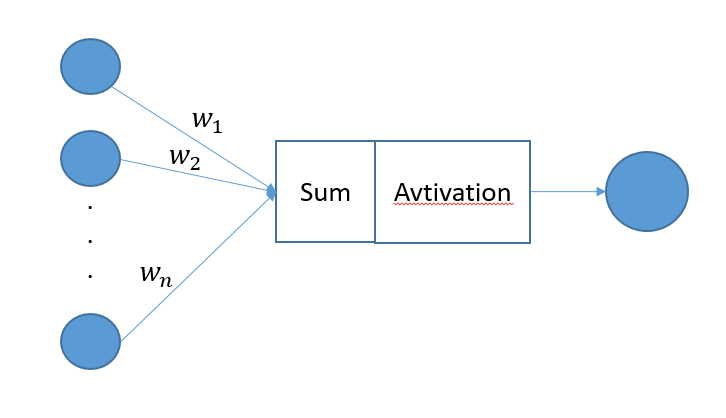
\includegraphics[width=\textwidth]{single.png}
			\caption{Input - Output}
			\label{fig:single}
		\end{subfigure}
		\hfill
		\begin{subfigure}[b]{0.49\textwidth}
			\centering
			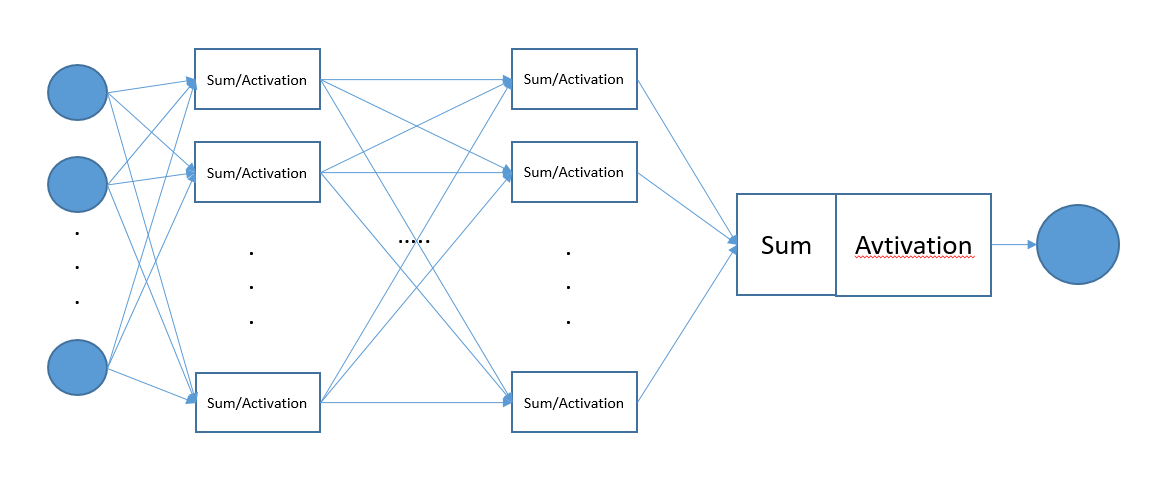
\includegraphics[width=\textwidth]{multiple.png}
			\caption{Multiple Hidden Layers}
			\label{fig:multiple}
		\end{subfigure}
		\caption{Neural Networks}
		\label{fig:neural_networks}
	\end{figure}
	
	Time series is a term that is defined as a sequence of values indexed with time. Machine learning can used in the context of time series to predict the next value in the future. Other applications regarding time series are classification in which model tries to classify a time series or a part of it and clustering in which model tries to group the data. Another application of using machine learning on time series data is the anomaly detection. In essence, much of real data is represented through time series which is data from systems, phenomena, or organs. If during the evolution (regarding time) of an operation, phenomenon or process there is something wrong then we get an anomaly. Then it is vital to get these points (anomalous points), and automatically recognize if a value is anomaly or not.
	
	The increase in the amount of data makes it difficult for humans to detect anomalies, and that is why we use algorithms to make the detection efficient and fast. It is therefore necessary to find models that detect "abnormalities" during the evolution of a process. There are many problems that anomaly detection tries to solve such as detecting bank fraud or early detection of tool malfunctions. Other applications relate to the health sector, such as the detection of various diseases or viruses. Applications also exist in industry such as fault detection or the detection of incorrect operation of a machine. Also money transactions and general fraud detection lies under the anomaly detection. These are just a few of the examples we can give in relation to anomaly detection.
	
	\section{Time Series and Stochastic Processes}
	
	In the study of phenomena, values emerge that appear in time sequence, one after the other. This family is called time series and formally we write $ X(t), t\in \mathbb{R}$. If for each moment we get more than one value we say that we have a multivariate time series and it is denoted by $  (X_i)_t, \quad t\in \mathbb{R}, \quad i\in \mathbb{I} $ where $X_{i,t}$ is the $i$ component of $Χ$ in time $t$. Otherwise, if for every moment we get a single value times series is called univariate time series. For example if we have a sensor that gives us a values for a phenomenon then the result will be a univariate time series. On the hand if we have many sensors then the result will be a multivariate time series. Len $\Omega$ be a sample space, we say that the family $X(\omega,t) $ where $t\in\mathbb{R}, \quad \omega \in \Omega$ is a stochastic process and for a moment of time $t\in \mathbb{R} $ the $X_t( \omega )$ is a random variable \cite{wei2006time}.
	
	A time series is said to have \textbf{Trend} if its mean $\mu$ is not constant and it increases or decreases with time. Also it is said that it has \textbf{Seasonality} if there is a periodic repetition of its fluctuations and is usually observed on an annual or monthly basis. Let be a time sereis, we define autocorrelation $\rho_\tau$ for a lag $\tau$ and the correlation coefficient two
	elements of the time series that are $\tau$ time steps apart and is estimated from the time series as
	
	$$ \rho_\tau = \text{Corr}(x_t, x_{t+\tau}) = E[(x_t-\mu)(x_{t+\tau}-\mu)] $$
	
	\noindent and correlation coefficient
	
	$$ r_\tau=\frac{\rho_\tau}{\rho_0} \quad , \quad -1\leq\rho_\tau\leq1$$
	
	\noindent Correlation make sense if time series is stationary.
	
	A time series that has no trend (ie has a mean of 0), no seasonality, constant variance, and constant autocorrelation is called \textbf{Στάσιμη} \cite{hyndman2018forecasting}. Noise $\epsilon_t$ is a stochastic process that is uncorrelated with time and comes from a distribution with constant mean $\mu=0$ and finite variance. Thus noise is a stationary stochastic process.
	
	\section{The problem of Anomaly Detection}
	The goal of Machine Learning is to identify the abnormal points of a time series in the future so that the necessary actions can be taken, for example if it is a fault, the fault should be fixed, or if it is an illegal entry into a system it should be dealt with. To go deeper into this problem we must first define what an Anomaly is. The term Anomaly is not easy to define. Therefore, several attempts have been made to define this term. According to Hawkins \cite{hawkins1980identification} an Anomaly is "an observation that deviates so significantly from other observations as to arouse suspicion that it was produced by some other mechanism". Then comes the term outlier. Many do not distinguish between these two terms and consider them equivalent. Thus we have definitions such as Grubbs \cite{grubbs1969procedures} who says that "Outlier observations, or outliers, are those which appear to deviate significantly from the other members of the sample in which they occur". And finally we get Aggarwal's definition which combines the two definitions into one as follows "Outlying points are often also referred to as non-normal, inconsistent, abnormal or anomalous, in the Data Mining and Statistics Literature". We will consider the term Anomaly to be equivalent to the term Outlier point. Here we have to distinguish the term Anomaly from the term Novelty which refers to data that is acceptable but does not resemble the rest of our sample \cite{Singh2003Novelty}. However, most algorithms are used to find both, so no further distinction will be made here. Finally, the main and most important problem in the definition of Anomaly is the concept of Noise. Noise are points that lie on the border between normal data and Anomalies, which could be called anomalies but are not points of interest. For this reason it is difficult to distinguish them Fig.~\ref{fig:anomaly vs anomaly with noise}. Some give the definitions \textit{Strong Anomaly} and \textit{Weak Anomaly} \cite{knorr1999finding} to distinguish the two concepts.
	
	\begin{figure}[h]
		\begin{subfigure}[b]{0.49\textwidth}
			\centering
			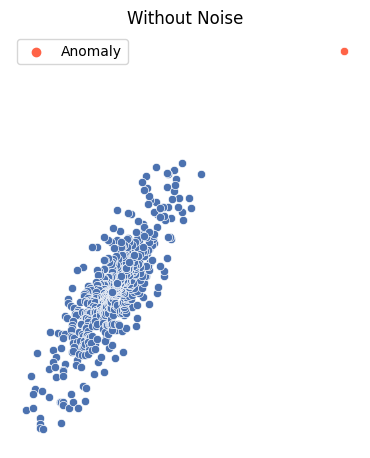
\includegraphics[width=\textwidth]{anomaly_vs_noise_clear_outlier.png}
			\caption{Anomaly without Noise}
			\label{fig:anomaly without noise}
		\end{subfigure}
		\hfill
		\begin{subfigure}[b]{0.49\textwidth}
			\centering
			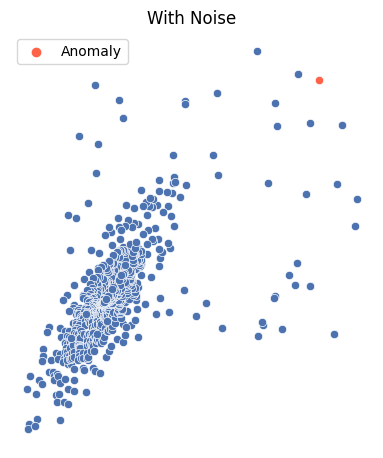
\includegraphics[width=\textwidth]{anomaly_vs_noise_no_clear_outlier.png}
			\caption{Anomaly with Noise}
			\label{fig:anomaly with noise}
		\end{subfigure}
		\caption{Anomaly with and without Noise}
		\label{fig:anomaly vs anomaly with noise}
	\end{figure}
	\noindent Thus, taking into account the above, we accept the following definition \cite{braei2020anomaly}:
	
	\begin{center}
		\textit{"An anomaly is an observation or sequence of observations that deviates significantly from the general distribution of the data. The total anomalies are a very small part of the total data."}
	\end{center}
	\hfill
	
	\section{Anomaly Types}
	
	Anomalies fall into three categories:
	
	\begin{itemize}
		\item \textbf{Point Anomalies} are called the points which deviate significantly from the rest of the sample. For example, a huge financial transaction that differs from the rest is called a Point Anomaly.
		
		\item \textbf{Collective Anomalies} are called the points which may be normal if we observe them individually but all together have an abnormal behavior. For example, if a customer of a bank withdraws 10 euros every 2 seconds from the bank, then these withdrawals are Collective Anomalies. 10 euros or 500 euros are normal amounts for a withdrawal but a series of such withdrawals is abnormal behavior.
		
		\item \textbf{Context Anomalies} or Context-dependent abnormalities are those points which are normal in a particular context but are reported as abnormal in another. For example the temperature $150 ^\circ C$ is a normal temperature for someone to cook their food in an oven but it is an abnormal value for the weather of a country.
	\end{itemize}
	
	\section{Anomaly Detection}
	
	Having defined what is an Anomaly, we can talk about Anomaly Detection. We define a function $ \varphi $ such that:
	\begin{align*}
		\varphi \colon \mathbb{R}^n \rightarrow \mathbb{R} \\
		\varphi(x)\mapsto\gamma
	\end{align*}
	where $ \gamma $ is Anomaly Score, $ x \in X \subseteq \mathbb{R}^n $ and $ X $ is the data set. Anomaly Score is defined as the measure to describe how much anomalous is a point, or how much this point deviates from the rest data set. We can transform it to a measure that belongs to interval $ [0,1] $ and then we can say that it is the probability of a point to be anomalous.
	
	To finally arrive at whether a point is an anomaly or not we define a threshold. A threshold is called a $ \delta \in \mathbb{R} $ , where all the points with an anomaly score below $ \delta $ will be the normal points while those with an anomaly score above $ \delta $ will be the anomalous points. Thus we define the binary anomaly detection method as:
	
	\begin{align*}
		\varphi_\text{binary} \colon \mathbb{R}^n \rightarrow \{Normal, Anomaly\} \quad \text{ή} \quad \{0,1\} \\
		\varphi_\text{binary}(x) \mapsto \begin{cases}
			Anomaly \quad \text{or} \quad 1, & \text{if} \quad \varphi(x) > \delta \\
			\phantom{-}Normal \quad \text{or} \quad 0, & \text{otherwise}
		\end{cases}
	\end{align*}
	
	Anomaly detection is not an ordinary two-class classification process. Naturally anomalies are less than 1\% which makes anomaly detection very different from two class classification. The difference lies in the fact that even if we say that all the points in a data set are normal points then the success of this model will be 99\%. But in reality the model will perform very poorly because it did not catch a single anomaly. For this reason we should tackle the problem with two well-known metrics: the F1 score and AUC (area under curve).
	
	$$ \text{Precision} = \frac{\text{TP}}{\text{TP}+\text{FP}}, \quad \text{Precision} = \frac{\text{TP}}{\text{TP}+\text{FN}} $$
	
	$$ \text{F}_1 = \frac{2 \cdot \text{Precision} \cdot \text{Recall}}{\text{Precision}+\text{Recall}} $$
	
	and
	
	$$ \text{TPR} = \frac{\text{TP}}{\text{TP}+\text{FN}}, \quad \text{FPR} = \frac{\text{FP}}{\text{FP}+\text{TN}} $$
	
	AUC is the area under the plot obtained by plotting on two vertical x,y axes, $ \text{FPR} $ on the x-axis and $ \text{TPR} $ on the y-axis. In essence, it shows how well the model can distinguish one class from another.
	
	Anomaly detection is not handled in the same way for all problems. Although we mentioned the difference in relation to two-class classification problems, we should say that anomaly detection problems (and thus their approaches) differ from each other depending on the type of anomalies they contain. This is clearly seen in the context of the time series we study in this thesis. For example, let's assume that we have a machine and we record in order among others the following temperatures in degrees Celsius: 35,34,34,35,36,37,36,90,92,92,93,92,94. If we approached the problem as if we had Point Anomalies then we probably wouldn't find any Anomalies because these temperatures are very normal for an engine. But if we take into account the time dependence of the temperatures then we observe an abnormal sudden rise from 36 degrees to 90. In the time series data we usually find Collective Anomalies or Anomalies that depend on the context (context anomalies).
	
	\chapter{Background}
	Anomaly detection is a subject that has many difficulties and is an evolving field. In the literature we will notice that the methods used can be categorized into 3 categories:
	
	\begin{itemize}
		\item Statistical methods
		\item Machine Learning methods
		\item Deep Learning methods
	\end{itemize}
	
	Statistical methods assume that anomalies generated from a statistical model. In contrast, in machine learning methods, the anomaly generation mechanism is considered as a black box and anomalies are detected based on the data. Finally, the third category concerns techniques based exclusively on neural networks, which are often considered part of Machine Learning, which is why there is often no separation between the second and third categories. Several methods have been presented by Markou, M. \& Singh, S. \cite{Singh2003Novelty, markou2003novelty} and by Chandola we have a very valuable research \cite{Chandola, chandola2009anomaly} who mentions algorithms of all three categories.
	
	\section{Statistical methods}
	
	\begin{itemize}
		\item \textbf{Autoregressive Model:}
		
		This model is considered linear where the value $X_t$ at time $t$ is based on the (finite) set of size $p$ of the previous values of the (stochastic) process and an error $\epsilon$, that is:
		
		$$X_t = \sum_{i=1}^{p}a_i X_{t-i} + c + \epsilon_t$$
		
		p is also called a window of length $p$ and the model is called an Autoregressive Model of order $p$ or simply $AR(p)$. The "error" values are considered uncorrelated and have mean $\mu=0$ and constant variance $\sigma$.
		
		The coefficients $a_1,....,a_p$ and $c$ can be approximated during training by solving the corresponding linear equations using the least square method. $\epsilon$ , which represents the anomaly score, can then be calculated as the difference between the "predicted" value and the actual value of X at time $t$ . The model assumes that the stochastic process is stationary, so if we do not have a stationary process then it should be transformed into one.
		
		\item \textbf{Moving Average Model:}
		
		While the previous model considers a $X_t$ value as a linear combination of the previous $p$ values, the Moving Average model considers this value as a linear combination of the previous $q$ forecasts' errors, so:
		
		$$X_t = \sum_{i=1}^{q}a_i \epsilon_{t-i} + \mu + \epsilon_t$$
		
		where $\mu$ is the mean value of X and the coefficients $a_1,....,a_q$ are calculated during training as before. $q$ is the size of the window and for this model (of order $q$) we write $MA(q)$. The difference with the previous model is that it considered the previous values from $X_t$ known, however in this model are considered unknown and predicted at each step thus producing the errors {$\epsilon_t,....\epsilon_{t-q}$}. 
		
		\item \textbf{Autoregressive Moving Average Model:}
		
		This model is a combination of the previous two and is often used on univariate time series data. denoted by $ARMA(p,q)$ and defined as:
		
		$$X_t = \sum_{i=1}^{p}a_i X_{t-i} + \sum_{i=1}^{q}b_i \epsilon_{t-i} + \epsilon_t$$
		
		$X(t)_{t\in\mathbb{R}}$ is an $ARMA(p,q)$ process if it is stationary. Actually this model uses fewer variables than the previous models but the main difficulty is in choosing the appropriate $p$ and $q$. The larger these values of these two parameters are, the more likely the model will be overfitted. This will result in many False Negatives, i.e. the model will not be able to recognize that something is an anomaly and decide that it is a normal point. On the other hand, if we choose very small values, we run the risk of getting many False Positives, i.e. the model will characterize several points as anomalies which in reality are not. In any case the model is not reliable.
		
		\item \textbf{ARIMA Model:}
		
		The major challenge faced by previous algorithms is that many processes are not stationary. This model addresses this problem by generalizing the Autoregressive Moving Average model by adding an additional parameter $d$ which defines how many times we will take the differences for a time series. That is:
		
		\begin{align*}
			d=0, & \quad X'_t = X_t \\
			d=1, & \quad X'_t = X_t-X_{t-1} \\ 
			d=2, & \quad X'_t = (X_t - X_{t-1}) - (X_{t-1} - X_{t-2})
		\end{align*}
		
		This transformation allows us to either remove the trend the time series may have, or to remove seasonality. It is applied as many times as we want until the time series is where we want it. Finally, the anomalous points are detected as in the previous algorithms (according to the error we get from the difference between the predicted value and the actual one).
		
		\item \textbf{Exponential Smoothing Model:}
		
		Unlike previous models that are linear, this model uses a non-linear approach. This model is defined as follows:
		
		$$ X_{t+1} = aX_t + a(1-a)X_{t-1} + a(1-a)^2X_{t-2},.....,+a(1-a)^NX_{t-N} $$
		
		where $a\in[0,1]$, so the prediction $X_{t+1}$ is a linear combination of the prior values with exponential weights. The parameter $a$ is called the weight reduction rate, and the smaller it is, the more weight is given to terms that are further away (regrading time). This model assumes that X is stationary.
		
		Variations exist to deal with non-stationarity by introducing additional parameters.
		
		\textbf{double exponential smoothing} 
		
		To deal with the problem of the trend in stochastic processes, the double exponential smoothing model is introduced, which is a generalization of the previous model. For the definition we have:
		
		\begin{align*}
			& S_0=X_0 \\
			& B_0=X_1-X_0 \\ 
			& \text{και} \\
			& S_t = aX_t + (1-a)(S_{t-1}+B_{t-1}) \\
			& B_t = \beta(S_t-S_{t-1}) + (1-\beta)B_{t-1}
		\end{align*}
		where $0\leq a\leq 1$ and $0\leq \beta\leq 1$
		
		and finally the model \textbf{triple exponential smoothing} is introduced to tackle the problem of seasonality \cite{HYNDMAN2002439}			
	\end{itemize}
	
	\section{Machine Learning methods}
	Machine learning methods try to detect anomalies without assuming that they come from a certain model. They rely on the fact that they don't need to know how the data was generated. So they are very different from the previous models.
	
	\begin{itemize}
		\item \textbf{K-Means Clustering}
		
		K-means may be a well-known algorithm in the context of unsupervised learning, however it can also be used in the context of anomaly detection. Let $(X_N)$ be a process, we first define a window of length $w$. Then we move the window by $\gamma$ and in each pass we get a subsequence. Thus a set such that  $\mathcal{S}\subseteq\mathbb{R}^{(N-w)\times w}$ is created with
		
		$$\mathcal{S} = \Bigl \{(X_0,X_1,...,X_w)^T , (X_{0+\gamma},X_{1+\gamma},...,X_{w\gamma})^T ,..., (X_{N-w},X_{N-w+1},...,X_{N})^T \Bigl \}$$
		
		k-means takes the number of clusters we want it to form as a parameter. After choosing this number, we apply the algorithm to the set $\mathcal{S}$ and the algorithm will calculate the centers of the clusters. Let $\mathcal{C}$ be the set of centers. Each subsequence from the set $\mathcal{S}$ belongs to a cluster, the distance from the center gives us a number which we define as the anomaly score. Thus for each subsequence the anomaly score $\epsilon_i = d(s_i,c_i)$ is defined, where $s_i\in\mathcal{S}$ and $c_i\in\mathcal{C}$. The distance $d$ is the distance function. Then anomalies are detected by setting a threshold $\delta$ and selecting every subsequence with a distance greater than this threshold to be an anomaly.
		
		Keogh and Jessica showed that this method is not reliable \cite{KeoghJessica2005}. This is because the centers of the clusters which selected are similar to the centers resulting from a process known as Random Walk. This means that we could get the centers from a Random walk instead of the $\mathcal{C}$ set we had before. Multiple experiments were done with different data sets and with different distances such as Manhattan, $L_\infty$ and Mahalanobis. In no experiment did a different result come out. This difficulty is to be explored and concerns many scientists. However, this algorithm is considered fundamental and for this reason a reference had to be made.
		
		\item \textbf{DBSCAN}
		
		Another algorithm used in clustering problems is DBSAN which is used for anomaly detection \cite{MartinKriegelXiaowei1996DBSCAN1996}. This algorithm is based on the density of points and has within it the concept of anomalies. That is, it divides the set of data into three categories: the main points, the border points and the anomalous points. The important parameters are two $\epsilon$ and $\mu$, which are the distance that defines whether a point is neighbor or not and the minimum number of points a cluster should have, respectively.
		
		So let a data set $\mathcal{S}$. The $\epsilon_\text{Neighbors}$ of a point $s_i\in\mathcal{S}$ is the set $\epsilon_\text{Neighbors}(s_i) = \Bigl \{s_j : s_j\in\mathcal{S}, \quad s_j\neq s_i, \quad d(s_i,s_j)\leq \epsilon \Bigl \} $, where $d$ is the distance function.
		
		A point is said to be Core point if $| \epsilon_\text{Neighbors}(s_i) | \geq \mu$.
		
		A point $s_i$ is Boundary point if 
		
		$$ \exists s_j \in \mathcal{S} : s_j\neq s_i, \quad s_j \in \epsilon_\text{Neighbors}(s_i), \quad | \epsilon_\text{Neighbors}(s_j) | = 1 $$  
		
		Finally, a point $s_i$ is an anomaly if it is none of the above, i.e. it is neither a core point nor a boundary point
		
		In time series data we can work in the same way as in k-means, i.e. by defining subsequences. The challenge in DBSCAN is to choose $\epsilon$ and $\mu$ appropriately.
		
		\item \textbf{Local Outlier Factor}
		
		The specific algorithm is not based on the density of the points but on the logic of the Nearest Neighbors, while at the same time it is based on the local outlier values (Local Outliers).
		
		Let $\mathcal{S}$ be the data set, for a point $s_i$ we define the LOF (local outlier factor) as follows:
		
		\begin{enumerate}
			\item \textbf{finding the set of $k$-Nearest Neighbors.} Let $k\in \mathbb{N}_+$. We calculate the distances of the points from $s_i$ and put them in order from smallest to largest. Then we choose the $k$-th distance. This distance is called $k-\text{distance}$ of $s_i$ and we write $\delta_k(s_i)$. So the set of $k$-Nearest Neighbors of $s_i$ is the
			
			$$N_k(s_i) = \Bigl \{ s \in \mathcal{S} : d(s_i,s) \leq \delta_k(s_i) \Bigl \} $$
			
			and the Reachability Distance of a point $s_j$ is 
			
			$$ RD_k(s_i,s_j) = max\{ \delta_k(s_j), d(s_i,s_j) \} $$
			
			\item \textbf{compute the Accessibility Density.} For a point $s_i$ the accessibility density of its $k-\text{distance}$ is
			
			$$LRD_k(s_i) = \Biggl ( \quad \frac{\sum\limits_{s\in N_k(s_i)}^{} RD_k(s_i,s)}{| N_k(s_i) |} \quad \Biggl )^{-1}$$
			
			\item \textbf{finally we can calculate the LOF.}  
			$$LOF(s_i)=\frac{\mathlarger{\sum}\limits_{s\in N_k(s_i)}^{} \frac{LRD_k(s)}{LRD_k(s_i)}}{| N_k(s_i) |}$$
		\end{enumerate}
		
		LOF is used as an anomaly score. So by setting a threshold we can decide whether a point is an anomaly or not.
		
		The difficulties we face with this algorithm are several. First we need to find the appropriate $k$ and the appropriate distance function $d$. Although the Euclidean distance works quite well many times it does not give us reliable results. Furthermore the algorithm refers to "locality". Another difficulty is that the time in the time series gives important information which is not exploited by the algorithm. Finally, it is computationally expensive because its complexity is $O(n^2)$.
		
		\item \textbf{Isolation Forest}
		
		\begin{figure}[h]
			\centering
			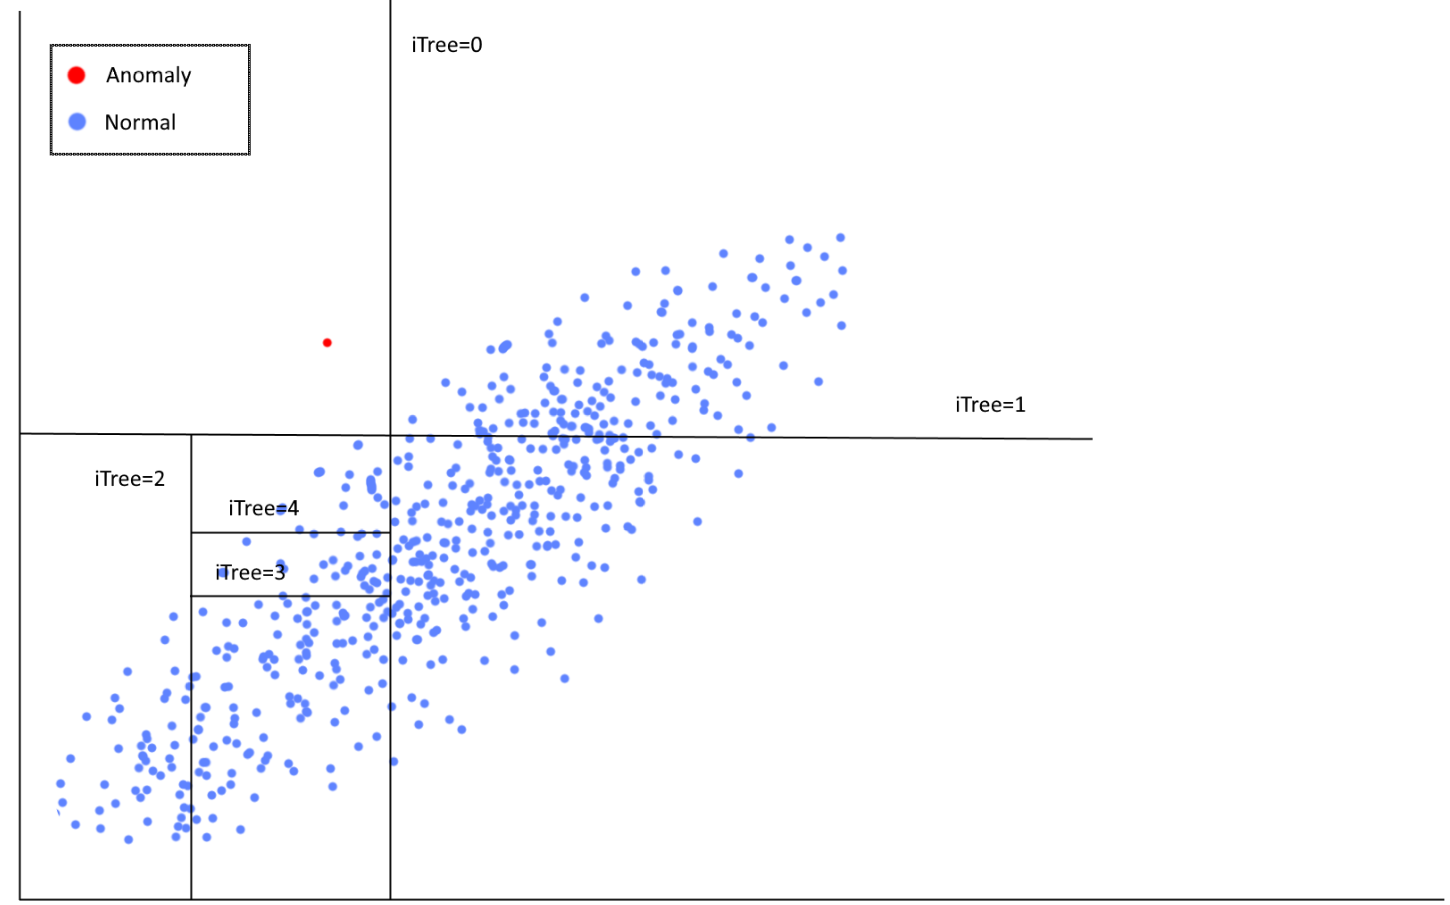
\includegraphics[width=\textwidth]{iTrees.png}
			\caption{Isolation Forest}
			\label{fig:iTrees}
		\end{figure}
		
		Isolation Forest was introduced by Liu \cite{TonyMingZhiHua2008IsolationForest} and is a method that divides the space multiple times until it isolates the points. It is an ensemble method that uses iTrees (which are a binary partition of space) to partition the space. Typically anomalies are isolated in just a few steps. In Fig.~\ref{fig:iTrees} we see an anomaly that was isolated in just 2 steps. In contrast, several steps are required to isolate normal points.
		
		The method is implemented in two steps: first we generate $n$ iTrees during training, and in the second phase which is called evaluation step we calculate the anomaly score.
		
		In order to apply Isolation Forest to the context of time series, we first need to define a window and then apply the algorithm to the set of subsequences. The anomaly score is derived from the average of the tree lengths, i.e. the depth of the Forest. 
		
		The main challenges of this method are three, the window size, the number of trees and the contamination parameter. If the window size is small then there will not be enough data to build a good model. On the other hand if it is large, then the oldest time data will have the same weight as the newest. Moreover, if the number of trees is large then it is closer to the expected value, however, the main problem is that the computational complexity increases because the algorithm runs in $O(Lw^2)$, where $L$ is the number of trees are constructed and $w$ is the window size. Finally, many implementations rely on a parameter called contamination, which indicates the percentage of anomalies that our data set contains. This parameter affects the threshold to detect anomalies so if we make a bad choice we risk getting a lot of false positives or false negatives.
		
		\item \textbf{Other techniques.}
		
		An interesting technique to mention is a variant of the SVM algorithm called \textbf{OC-SVM} \cite{vapnik1964class, ocsvm1999anomalydetection} which is an SVM algorithm configured to applied for a One Class problem. Finally we have the well-known algorithm \\ \textbf{XGBoost} which is a Boosting technique \cite{Chen_2016}.
	\end{itemize}
	
	\section{Deep Learning methods}
	These methods are similar to Machine Learning methods because they do not consider that the data derived from some mechanism on the background. They consider the mechanism as a black box and try to make predictions empirically. We decide to separate machine learning and deep learning methods as the latter focuses on neural network exclusively, although many researchers do not distinguish them.
	
	\begin{itemize}
		\item \textbf{Multiple Layer Perceptron.}
		
		The most basic neural network architecture is the MLP. Here we will define a window of length $w$. Then we will take the subsequences and predict as follows: for the subsequence $(x_{i-w}, x_{i-w+1}, ... , x_{i})$ we can predict the next value $\hat{y} = f(x_{i+1}) $. Alternatively we can predict a longer interval of length $m$, $\hat{y} = f((x_{i+1}, x_{i+2},....,x_{i+m}))$. The interval length $m$ is called the prediction window.
		
		To detect anomalies we set a threshold $\delta$ and for each prediction we get the error $\epsilon_i = \hat{y_i} - x_i $ which will be used as an anomaly score. So:
		
		\begin{equation*}
			\varphi(x_i) = \begin{cases}
				1 &,\text{ If } \epsilon_i\geq\delta\\
				0 &, \text{ Otherwise}
			\end{cases}
		\end{equation*}
		
		This algorithm has many parameters and therefore several challenges. First we have the depth of the network and its width, i.e. the number of hidden layers and the number of nodes in each layer respectively. Next we should define the length of the window and finally we have the optimization function.
		
		\item \textbf{Convolutional Neural Networks}
		Convolutional neural networks have been very successful in the field of image recognition, object recognition, categorization, etc. However, we can also use them in anomaly detection. Unlike MLP networks which are fully connected (so we have many weights) convolutional networks are partially connected which allows them to have fewer variables to calculate, making them faster to train while allowing them to have more depth. In addition, these networks use a technique called pooling to avoid overfitting. Another frequently used technique is called Batch Normalization \cite{SergeyChristian2015BatchNormalization} which is an alternative to dropout i.e. it reduces the importance of initializing values. 
		
		To train a Convolutional Network a filter is applied (an array i.e. $n\times k$, which is typically $3\times 3$, $5\times 5$, etc) which is shifted to scan all the data and apply the operator of convolution Fig.~\ref{fig:convfilters}.
		
		\begin{figure}[h]
			\centering
			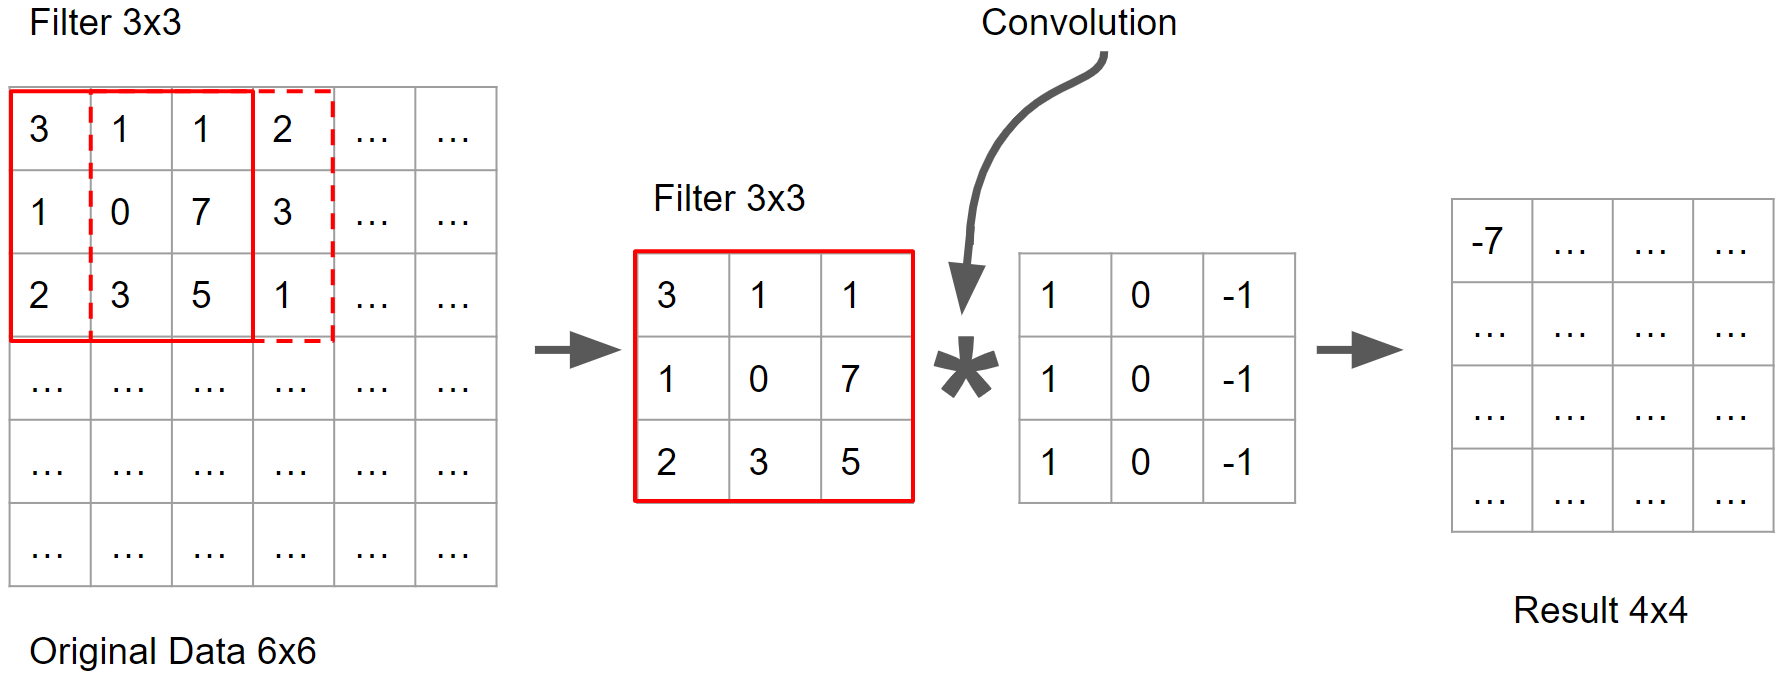
\includegraphics[width=\textwidth/8*7]{convfilters.png}
			\caption{Filter of Convolutonal Layer}
			\label{fig:convfilters}
		\end{figure}
		
		The use of convolutional in anomaly detection is done in the same way as before, i.e. we define a window and the training is done on the subsequences. The detection is done by defining a threshold and finally the decision is made on the errors between the predictions and the actual value, i.e. we have an anomaly if $f((x_{i-w}, x_{i-w+1}, ... , x_{i}))-x_{i+1} \geq \delta$
		
		The challenges faced by this method are primarily the architecture of the network. Here we have a difficulty because the architecture of the network is very influential in the final prediction, for example it matters a lot if we will use dropout, Batch Normalization and/or max-pooling. In addition, the number and size of the kernels to be used in each convolutional level matters. Kernel is called a filter that scans a convolutional layer which extracts various features. Finally, an important factor is the depth which should be decided when defining the network.
		
		\item \textbf{Residual Neural Network}
		
		\begin{figure}[h]
			\centering
			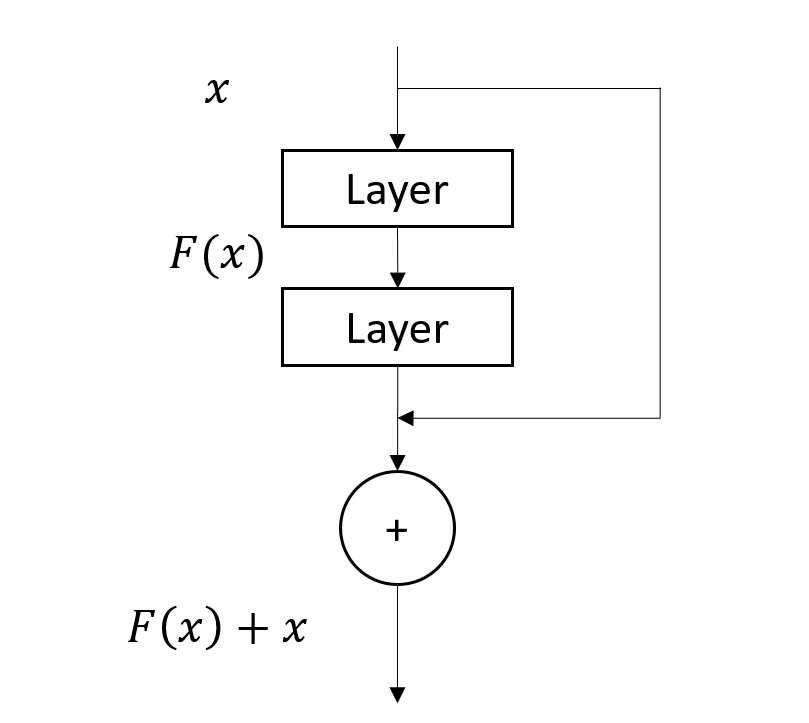
\includegraphics[width=\textwidth/2]{resnetplus.png}
			\caption{Residual Network}
			\label{fig:resnetplus}
		\end{figure}
		
		Residual networks are an extension of Convolutional. These networks combine a result from the previous levels with the result of a later level Fig.~\ref{fig:iTrees} this block is called a residual block \cite{HeZhangRen2015Residual}. To define a residual block we consider $x$ as its input, and $\varphi$ a convolutional block, which consists of convolutional layers, max-pooling, batch normalization, etc. The output of a residual block is $y=x+ \varphi(x)$. Usually an activation function $\varPsi$ is also included and finally we have $y=\varPsi(x+\varphi(x))$.
		
		Residuals networks are used to solve the "vanishing derivative" or the "vanishing gradient" problem that arises from Convolutional networks due to their depth. In essence, this problem refers to derivatives which are so small that they essentially zero (vanish) so they preventing the weight from changing its value.
		
		\item \textbf{LSTM - Long Short Term Memory Network.}
		
		A network known for its application to sequential data is the LSTM network which belongs to the family of Recurrent Neural Networks. Unlike the previous ones where the data had a continuous path forward, a Recurrent network has a connection with the data that has already passed, which allows it to draw information according to other data and combine knowledge. So formally the output produced is the following:
		
		$$ y_i = h({x_i}^T \cdot {w_x} + {y_{i-1}}^T\cdot {w_y} + b)$$
		
		where $h$ is the activation function, $x_i$ is an element from the data set, $y_{i-1}$ is a "previous" predicted value, $w_x, w_y$ are the weights, and $b$ is a constant.
		
		\begin{figure}[h]
			\centering
			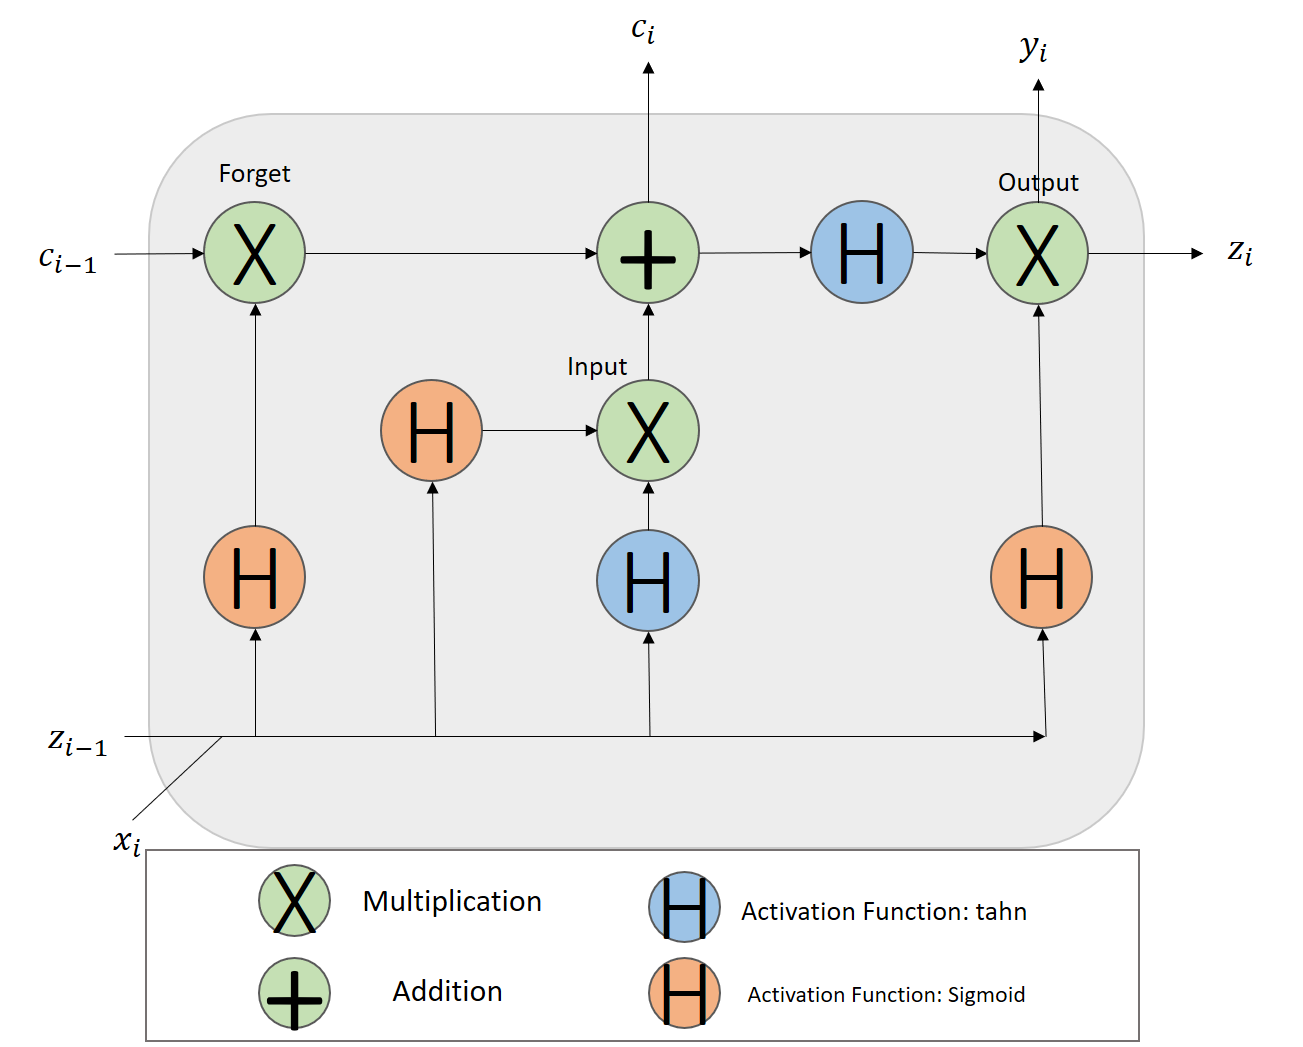
\includegraphics[width=\textwidth]{lstmarchitecture2.png}
			\caption{LSTM}
			\label{fig:lstmarchitecture}
		\end{figure}
		
		An LSTM network is therefore a variant of such a network \cite{LSTM1997HochreiterSchmidhuber} in which two vectors $c_i$ and $z_i$ are included. $z_i$ is added with $x_i$ and is called short term while $c_i$ is multiplied with $x_i$ and is called long term. In addition there are 3 "gates" that regulate the information,  Forget Gate that will thrown away any information that is not useful, the input gate that will pass the information, and the output gate that will be the output of the new information. This design has the effect of storing important information during addition to be used later (long term) and by using multiplication (point wise) it is possible to delete information that is useless according to the model from the long-term term. Finally the output gate decides which part of the long-term term will be the output Fig.~\ref{fig:lstmarchitecture}.
		
		The steps LSTM performs are as follows:
		
		\begin{enumerate}
			\item First we will be transferred to the forget gate where it will be decided what information will be thrown away. It takes the input $x_i$ and the previous output $z_{i-1}$, and with the help of a Sigmoid activation function (let $h_s$) we have $f_i = h_s(W_f\cdot [ z_{i-1, x_i}] + b_f)$. As a last step when we go to the forget gate we multiply by the old state and we have $F_i = f_i \cdot C_{i-1}$
			\item Then it is decided what information to hold (input gate). First a sigmoid activation function is applied to the input $x_i$ and the previous output $z_{i-1}$ which will decide which values should be updated $u_i = h_s(W_u \cdot [z_{i-1}, x_i] + b_u)$. And secondly a tanh activation function will be applied (let $h_\text{tanh}$), $\hat{C_i} = h_\text{tanh}(W_C \cdot [z_{i-1}, x_i] + b_C) $ for update. Finally we will get, after applying the input gate, $I_i = u_i \cdot \hat{C_i}$
			\item Then we combine the two previous steps. We apply an addition and we have $ C_i = F_i + I_i$
			\item Since the previous steps have been taken now is the time to decide the output. First we pass the previous result from the tanh activation function to limit the values in the interval -1, 1 by taking $r_i = h_\text{tanh}(C_i)$ and then we will pass the input $x_i$ and the previous output from sigmoid activation function to get $o_i = h_s(W_o \cdot [z_{i-1}, x_i] + b_o)$. After the multiplication we will get the output from the gate output $O_i = o_i \cdot r_i$
			\item during this process the values of $C_i$, $O_i=z_i$ are saved for future use
		\end{enumerate}
		
		\item \textbf{Autoencoder.}
		
		The autoencoder method is implemented in two steps. In the first step the model encodes the input and in the second step it decodes the input Fig.~\ref{fig:autoencoder}. The main idea behind this algorithm is that if we project the points into a smaller dimensional space the normal data will be significantly different from the anomalies. So if we do the reverse process, the points that have significant differences compared to their initial state will be anomalies. This concept makes the autoencoder a very good choice for anomaly detection.
		
		\begin{figure}[h]
			\centering
			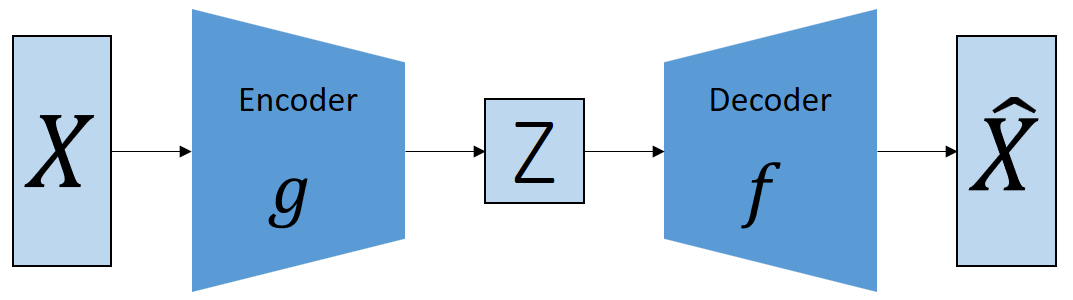
\includegraphics[width=\textwidth]{autoencoder.png}
			\caption{Autoencoder}
			\label{fig:autoencoder}
		\end{figure}
		
		Such networks belong to the family of feed-forward networks (as was the MLP algorithm we saw earlier) in contrast to LSTMs. The first step of the process is called the encoder (Encoder) while the second step is called the decoder (Decoder). We formally have:
		
		Let $\mathcal{X}$ be the data set, $f$ the decoder function and $g$ the encoder function, we have:
		
		$$\hat{X} = f(g(X))$$
		
		The optimization function will try to minimize the difference between $\hat{X}$ and $X$ , that is:
		
		$$\min_{w_f, w_g} \lvert \lvert X - \hat{X} \rvert \rvert_2  = \min_{w_f, w_g} \lvert \lvert X - f(g(X)) \rvert \rvert_2$$
		
		Finally from each $x_i$ we get a $\hat{x_i}$ and we have the error $\epsilon = \lvert x_i - \hat{x_i} \rvert$ which we use as an anomaly score. By setting a threshold $\delta$ we can decide what is an anomaly and what is not.
		
		Autoencoders are often combined with other networks, for example CNN networks or LSTMs. With this composition, these networks take the role of encoder/decoder and the result is to get the advantages of both techniques. The process is as follows: first the data goes through the network (first step Encoding) to reduce the dimensions and then to the same network with the reverse architecture (second step Decoding) to get back an element of the original space. Anomalies are detected as we said before.
		
		\item \textbf{Variational Autoencoder και LSTM-VAE}
		
		\begin{figure}[h]
			\centering
			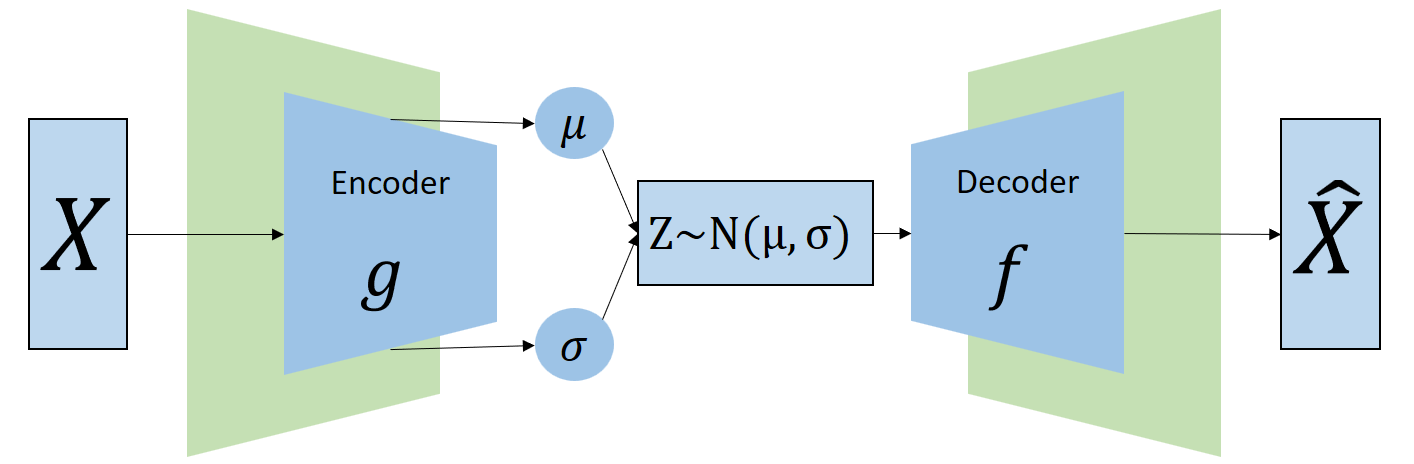
\includegraphics[width=\textwidth/8*7]{lstmvae.png}
			\caption{LSTM-VAE}
			\label{fig:lstmvae}
		\end{figure}
		
		A variant of the autoencoder is the Variational autoencoder (or Auto-Encoding Variational Bayes \cite{Kingma2013WellingVAE}) where a Z is sampled from a normal distribution, while the encoder and decoder are the posterior $q(z;x)$ and the prior $p(\hat{x};z)$.
		
		The LSTM-VAE network combines a Variational Autoencoder with an LSTM Fig.~\ref{fig:lstmvae} which is actually a variant of LSTM-AE.
		
		
		\item \textbf{Other techniques.}
		
		Furthermore before closing this section we should make a reference to networks worth mentioning such as WaveNet \cite{Oord2016WaveNet} and a variant of LSTM called GRU \cite{ChoMerrienboer2014GRURNN}. In the case of WaveNet the time series is imported just like in a convolutional network, defining a window which defines subsequences which in turn are given to the model. The main difference between WaveNet and convolutional is that WaveNet uses dilation filters Fig.~\ref{fig:dilationfilters}. 
		
		\begin{figure}[h]
			\begin{subfigure}[b]{0.4\textwidth}
				\centering
				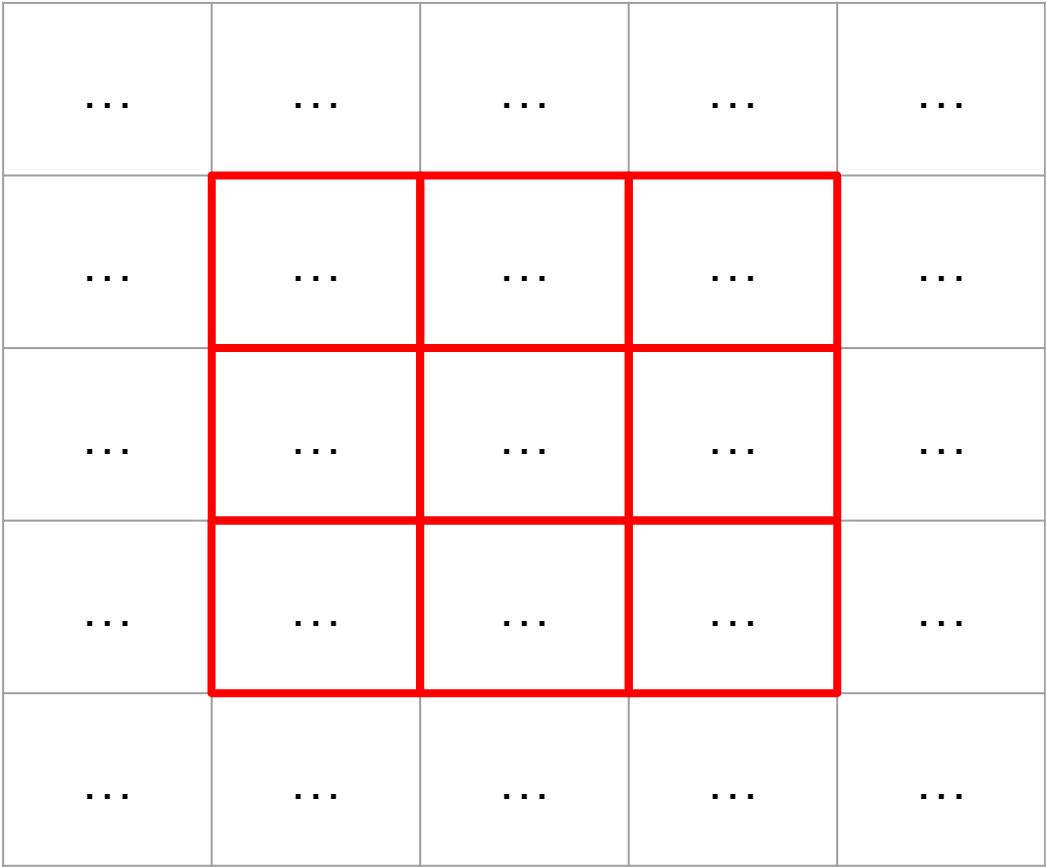
\includegraphics[width=\textwidth]{dilationfilters_withoutdilation.png}
				\caption{Without dilation}
				\label{fig:dilationfilters_withoutdilation}
			\end{subfigure}
			\hfill
			\begin{subfigure}[b]{0.4\textwidth}
				\centering
				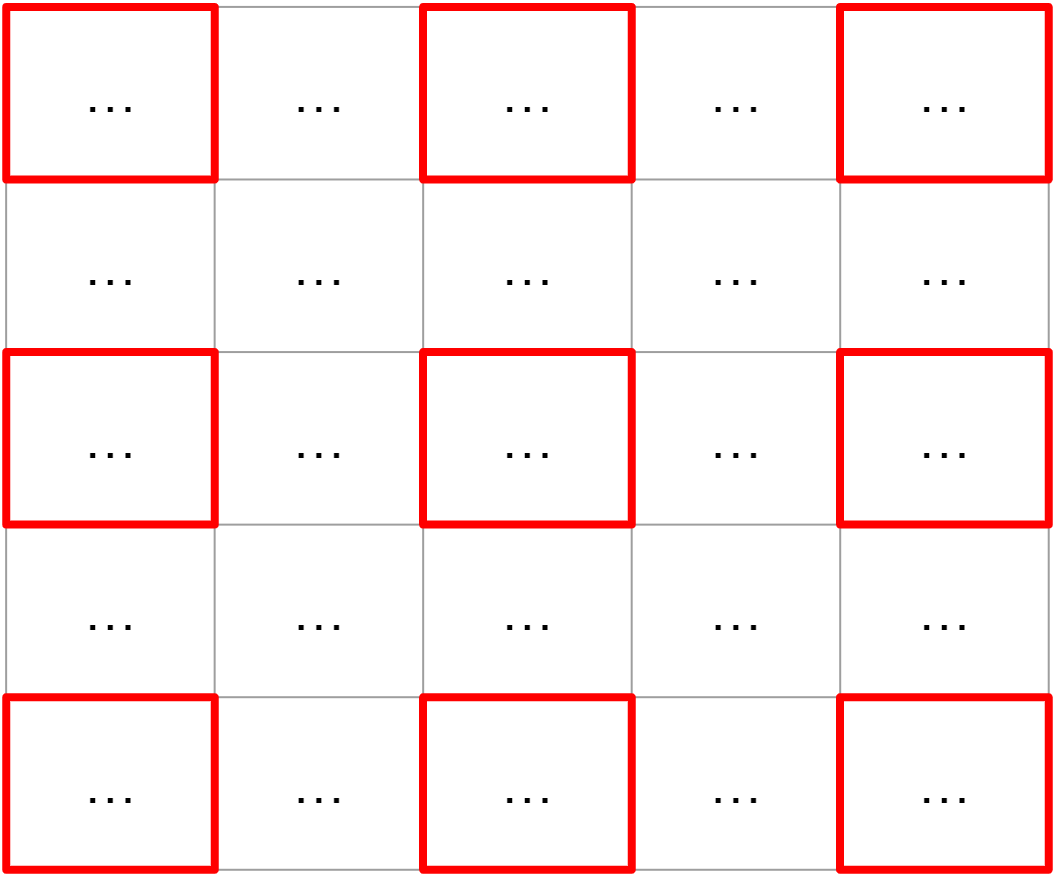
\includegraphics[width=\textwidth]{dilationfilters_withdilation.png}
				\caption{With dilation}
				\label{fig:dilationfilters_withdilation}
			\end{subfigure}
			\caption{no dilation vs dilation}
			\label{fig:dilationfilters}
		\end{figure}
		
		Από την άλλη το GRU είναι μία παραλλαγή του LSTM, οι χρονοσειρές εισάγονται κατά τον ίδιο τρόπο με το LSTM ορίζοντας ένα παράθυρο μήκους $w$. Η ομοιότητα με το LSTM είναι μεγάλη και στη βιβλιογραφία φαίνεται να έχουν τις ίδιες επιδόσεις. Η μεγαλύτερη διαφορά είναι ότι το GRU έχει πιο απλή δομή Fig.~\ref{fig:lstmgrucomparison}. Ως εκ τούτου έχει λιγότερες μεταβλητές και άρα εκπαιδεύεται σε λιγότερο χρόνο.
		
		\begin{figure}[h]
			\centering
			\begin{subfigure}[b]{0.8\textwidth}
				\centering
				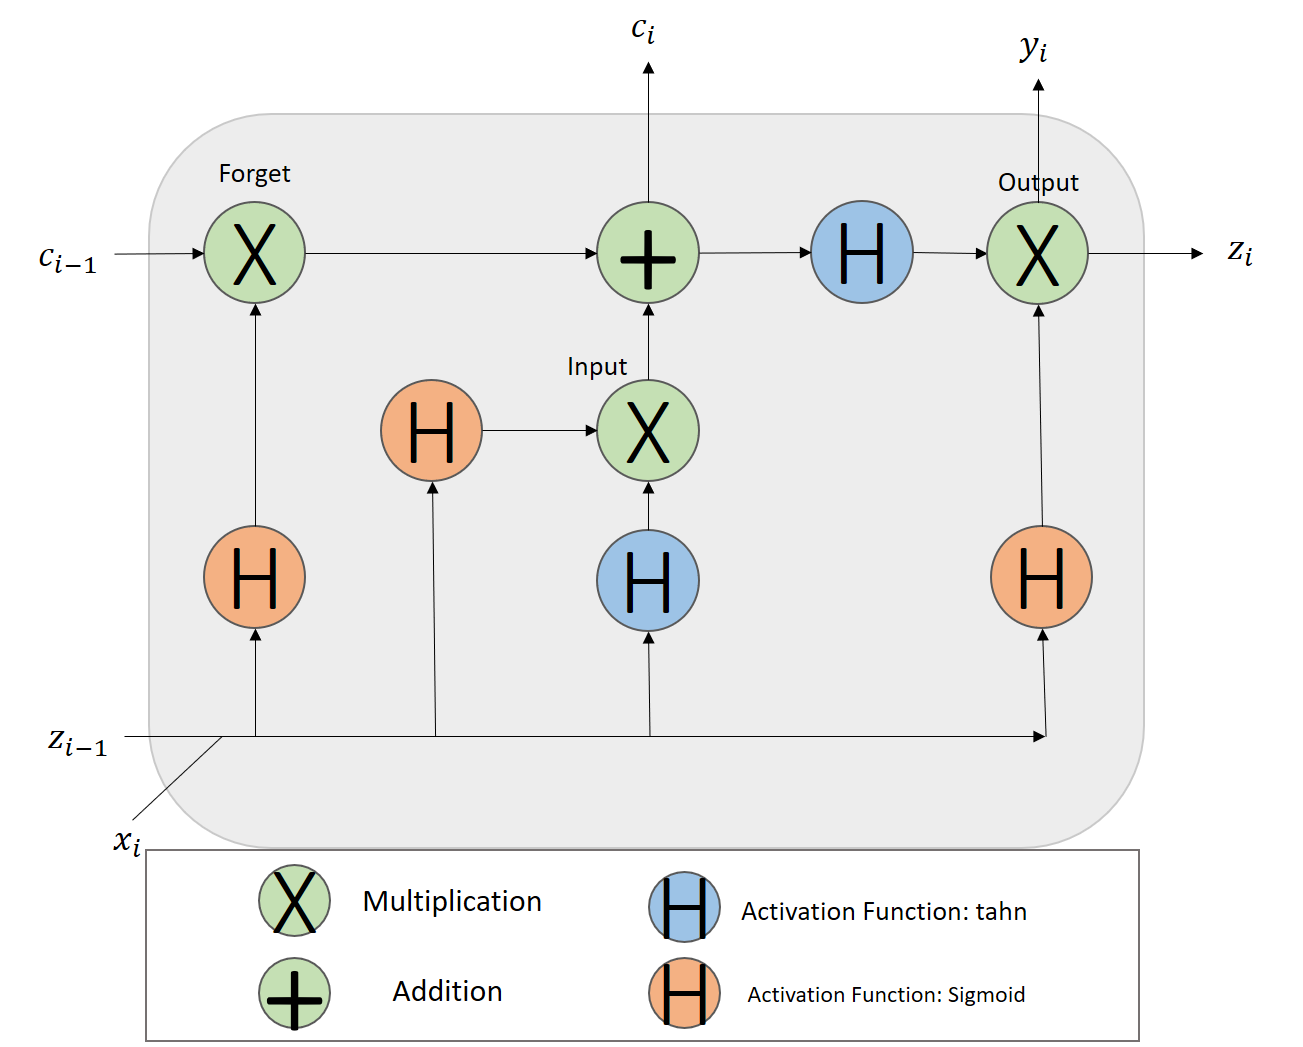
\includegraphics[width=\textwidth]{lstmarchitecture2.png}
				\caption{LSTM}
				\label{fig:lstmarchitecturecell}
			\end{subfigure}
			\hfill
			\begin{subfigure}[b]{0.8\textwidth}
				\centering
				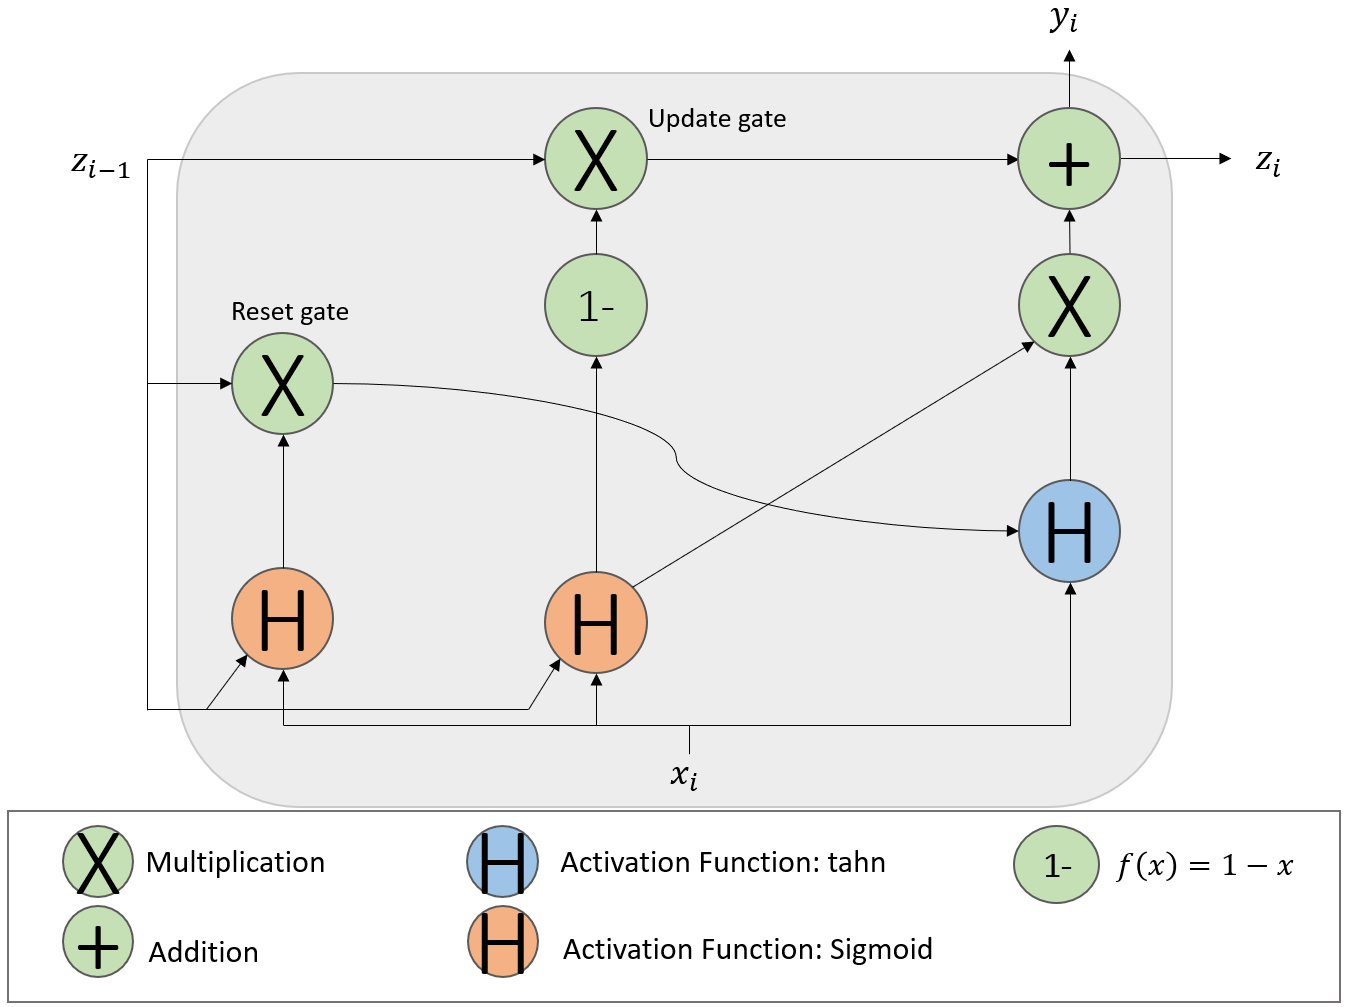
\includegraphics[width=\textwidth]{gruarchitecture2.png}
				\caption{GRU}
				\label{fig:gruarchitecturecell}
			\end{subfigure}
			\caption{LSTM cell vs GRU cell}
			\label{fig:lstmgrucomparison}
		\end{figure}
		
	\end{itemize}
	
	
	\chapter{Outlier detection in time series data using ensemble techniques}
	\section{Ensemble}
	In this chapter we will see some ensemble techniques which will be compared with the basic algorithms on which they are based. Machine learning methods based on other models are called Ensemble. In essence, they aggregate the results of other models and combine them into a final result. The group of models and their combination is called Ensemble. Ensemble models have been widely used in various types of problems, such as categorization or price prediction. Well-known algorithms like Random Forest and Majority Voting are very successful in this kind of problems. But also more complex algorithms like Bagging, boosting and Stacking have been used a lot. The bagging method consists of two steps. In the first step we have some initial models and select only some of the data for each model to train on a limited number of observations. So, in a sense, each model finds different patterns in the data set. In the second step, we gather the results and arrive at a forecast which results from the combination of the individual forecasts. In the boosting method we train the models in sequence one after the other, giving one model the output of the previous one. Thus, a model is trained from the mistakes of its predecessor, as a result as the process progresses, the models that are towards the end become more powerful. In the stacking technique, unlike boosting, all models are trained in parallel, while the difference with the bagging technique is that the training of all models is done on all data from the training dataset. At the final stage of a stacking technique there is a model that will be trained to correctly combine the results of the other models. The final model is called the meta-learner or the meta-model. 
	
	Although ensemble techniques are widespread, in the field of anomaly detection in multivariate time series they have not been studied as much. In this dissertation we give ensemble techniques that have been used for other kinds of problems while at the same time comparing the results with the basic algorithms used to compose the ensembles. We will also give an implementation that was not found in the anomaly detection literature, at least as far as our personal search is concerned. Eventually we will use the above techniques such as bagging and stacking. First we will create models by the bagging technique and then we will give their outputs to a meta-model according to the stacking technique. 
	
	In the following ensemble techniques we have used the same models everywhere which are: Autoencoder, LSTM, Autoencoder with LSTM (LSTM-AE), Convolutional Autoencoder (CONV-AE) and an LSTM-VAE.
	\section{Data}
	
	The datasets used are taken from SKAB (Skoltech Anomaly Benchmark) \cite{skabdataset}. The datasets have been produced by a device which includes:
	
	\begin{itemize}
		\item A water circulation system.
		\item A water circulation control system.
		\item A system for monitoring the condition of water in the circulation system.
		\item A technology (TSN) for recording time.
		\item Finally a system for data storage.
	\end{itemize}
	Also, this device has valves and mechanisms to create abnormal operation and sensors to capture the values.
	
	The data are multivariate time series. Each line within the dataset symbolizes a record of a given moment in time which consists of 8 variables, the moment in time when the observation was made and the indication if it is an anomaly or not:
	
	\begin{itemize}
		\item datetime - Is the time when the observation is recorded.
		\item Accelerometer1RMS - Acceleration (unit g)
		\item Accelerometer2RMS - Acceleration (unit g)
		\item Current - Shows the current (ampere unit)
		\item Pressure - Pressure (unit Bar)
		\item Temperature - Temperature (Degrees Celsius)
		\item Thermocouple - Temperature (Degrees Celsius)
		\item Voltage - The volts of the machine (Volt unit)
		\item RateRMS - Rate of flow of fluid in the loop (Unit Liters/Minute)
		\item anomaly - Indicates if the point is an anomaly (0 or 1)
	\end{itemize}
	
	The data simulates various situations (each data set describes a different situation and we have selected 31 data sets in total) such as Simulate liquid leakage and addition, Sudden unbalance behavior, Sudden liquid increase/decrease, Slow liquid increase, High temperature liquid increase and others. Depending on the case, a different set of data has been created where initially the system works in normal conditions and then a scenario is simulated where we observe the anomalies.
	
	SKAB is therefore a collection of data that can be used to evaluate techniques and models in the context of Anomaly Detection research in multivariate time series. The authors at \cite{skabdataset} have experimented with several of the models we have already described such as Convolutional Autoencoder, LSTM, LSTM Variational Autoencoder, Isolation forest and others. The results they achieved show that they achieve 0.79 F1-Score with Convolutional Autoencoder in first place while Isolation Forest is in last place with 0.4 F1-Score, Table~\ref{tab:skabresults}. In \cite{elhalwagy2022hybridization} a new Neural Network architecture is proposed which results in a hybrid Network derived from Capsule and LSTM networks. The authors use the SKAB datasets to evaluate their architecture. Here we observe the results to be with an LSTMCaps in first place with 0.74 F1-Score while Isolation Forest is in last place with 0.4 F1-Score Table~\ref{tab:capsuleandlstm}. Finally in \cite{pranavan2022contrastive} a model called TRL-CPC is proposed which learns to represent the time series through Contrastive Learning. Contrastive Learning is called the training of a model where the samples are compared with each other and the model learns to find the similarities of the characteristics of the samples belonging to the same class. The authors manage to achieve a 0.70 F1-Score with TRL-CPC on the SKAB dataset.  
	
	\begin{table}[H]
		\begin{subtable}[h]{0.31\textwidth}
			\centering
			\resizebox{\textwidth}{!}{
				\begin{tabular}{|c|c|}
					\hline
					Model Title & F1 Score \\
					\hline
					Conv-AE & 0.79 \\
					\hline
					MSET & 0.73 \\
					\hline
					LSTM-AE & 0.68 \\
					\hline
					T-squared+Q (PCA) & 0.67 \\
					\hline
					LSTM & 0.64 \\
					\hline
					MSCRED & 0.64 \\
					\hline
					LSTM-VAE & 0.56 \\
					\hline
					T-squared & 0.56 \\
					\hline
					Autoencoder & 0.45 \\
					\hline
					Isolation forest & 0.4 \\
					\hline
				\end{tabular}
			}
			\caption{SKAB Results}
			\label{tab:skabresults}
		\end{subtable}
		\hfill
		\begin{subtable}[h]{0.31\textwidth}
			\centering
			\resizebox{\textwidth}{!}{
				\begin{tabular}{|c|c|}
					\hline
					Model Title & F1 Score \\
					\hline
					LSTMCaps & 0.74 \\
					\hline
					MSET & 0.73 \\
					\hline
					LSTMCapsV2 & 0.71 \\
					\hline
					MSCRED & 0.7 \\
					\hline
					LSTM & 0.67 \\
					\hline
					Conv-AE & 0.66 \\
					\hline
					LSTM-AE & 0.65 \\
					\hline
					LSTM-VAE & 0.56 \\
					\hline
					Autoencoder & 0.45 \\
					\hline
					Isolation forest & 0.4 \\
					\hline
				\end{tabular}
			}
			\caption{Hybridization of Capsule and LSTM Networks}
			\label{tab:capsuleandlstm}
		\end{subtable}
		\caption{Results from related work}
		\label{tab:otherresearchresults}
	\end{table}
	
	\section{Majority Voting}
	The logic of Majoriy Voting is based on the following: If we ask a question to 1000 people then it is more likely that the majority will find the correct answer. This is called "the wisdom of the majority". In mathematics this is shown with the help of the binomial distribution: Let $X_i$ be independent and equal random variables with $ X_i \sim bernoulli(p), \quad i=1,2,....,1000$ where the probability of a correct answer is $ p=51\% $. The $X_i$ correspond to humans and the probability 51\% corresponds to their ability to answer correctly. That is, they are little better than responding to chance by flipping a coin. Then the probability that more than half answer correctly is $P(X\geq501) = 1-P(X\leq500)$. From the binomial distribution we know that $P(X\leq500) = \mathlarger{\sum\limits_{n=0}^{499}} \mathlarger{\binom{\mathlarger{1000}}{\mathlarger{n}} } (\frac{51}{100})^n(1-\frac{51}{100})^{1000-n} \approx 25\%$. So we have that $P(X\geq 501)\approx75\%$. Which means we have a 75\% chance that more than 500 people will answer correctly. The more people we increase, the more this probability grows (for example, if we have 10000 people, this probability is close to 97\%).
	
	In this technique we use all the models mentioned above in this chapter as basic prediction models, which are much better than a simple 51\% in their predictions. The process is:
	
	\begin{enumerate}
		\item We train all models on a piece of our data.
		\item We then make predictions on all our data. For each point each base model produces a label (if anomaly then 1 otherwise 0)
		\item For each point we have a 5-vector $(X_1, X_2, X_3, X_4, X_5)$ where $X_i \in \{0,1\}$ denote the label given by the algorithm $i$ to this point .
		\item If the 1's are more than the 0's then the point is characterized as an anomaly.
	\end{enumerate}

	\begin{figure}[h]
		\centering
		\includegraphics[width=\textwidth]{majorityvotingpc.png}
		\caption{Majority Voting}
		\label{fig:majorityvotingpc}
	\end{figure}

	
	
	According to this algorithm if a model fails to fit some data set while the other algorithms do better then the point will not be lost and if it is an anomaly it will be detected Fig.~\ref{fig:majorityvotingpc}. Due to the nature of the anomalies, the data sets have several differences between them. This would result in an algorithm alone being able to see some patterns in some sets while failing in others. The Majority Voting method solves this problem by using knowledge from 5 different models. This algorithm can be used with a variation and give a weight to the answers of the basic algorithms, then depending on the weight the final conclusion will be made. We chose to keep giving each algorithm the same weight so all answers count the same. Below is a more advanced variant of this algorithm.
	
	\section{Logistic Regression}
	This method is very popular in categorization. Here we will use this method in the semi-supervised learning environment where we will first train the basic models and then train a logistic regression model on the anomaly scores we have extracted from the models. In essence, we want our model to learn to combine the knowledge given to it by the basic algorithms so that it can predict whether a point is an anomaly.
	
	\begin{figure}[h]
		\centering
		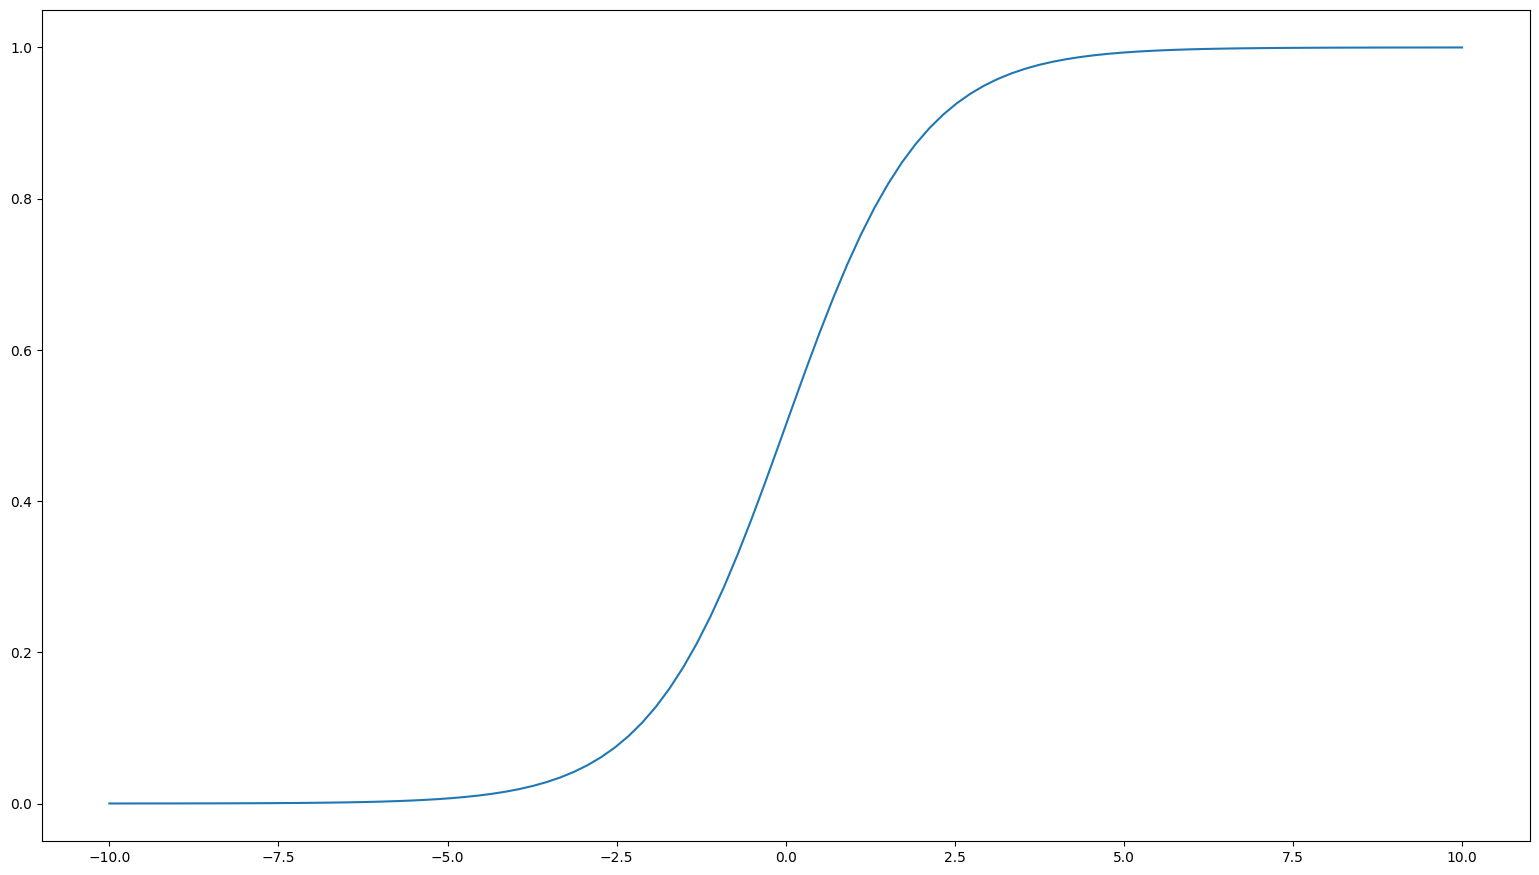
\includegraphics[width=\textwidth]{sigmoid.png}
		\caption{Sigmoid}
		\label{fig:sigmoid}
	\end{figure}
	
	The logistic regression model uses the sigmoid function Fig.~\ref{fig:sigmoid} which is $\sigma(x) = \frac{1}{1+\exp(-x)}$. The algorithm estimates the probability $\hat{p}=\sigma(X^T\theta)$ and the prediction is
	\begin{equation*}
		\hat{y} = \begin{cases}
			0, &\hat{p}<0.5\\
			1, &\hat{p}\geq 0.5
		\end{cases}
	\end{equation*}
	
	The ensemble method is therefore performed in two steps.
	\begin{itemize}
		\item First we take a piece of the data for training and divide it into two subsets that are disjoint, let be $A$ and $B$
		\item We then train the base models on set $A$ without seeing set $B$ at all. This is done so that there is no information leakage between the models and the logistic regression.
		\item We then make predictions on the set $B$ with the basic models and build a set $B'$. Thus, our set consists of elements whose dimensions are the predictions of the basic models.
		\item Finally we train the logistic regressor on the elements of $B'$ giving it their real labels at the same time (for this reason it is called semi-supervised learning).
	\end{itemize}
	Eventually the logistic regression will have learned to rely on the predictions of the basic models. However, by keeping the training of the basic models and the training of the logistic regression separately, we actually manage to give the predictions of each basic model a weight. Combined that is, in the end if a model is not that reliable, logistic regression will not get much of its opinion unlike in the previous method (Majoriy Voting) where each model was treated the same as the rest (giving a weight of 1 to all).
	
	The anomaly finally results from the probability extracted after the prediction according to what we have shown above. That is, a value below 0.5 is a normal point, while a value above 0.5 is an anomalous point. Depending on the case we could change the 0.5 threshold to move the decision boundary. This would give us more False Positives or False Negatives if we lowered or raised the threshold. For example, if we are dealing with diseases in a population, we would ideally like our model not to characterize something as normal when in fact it is not which means we want to decrease the false negatives. In the example we gave a low threshold would be better suited because it is very harmful for something dangerous to pass. On the other hand it isn't big deal if we categorize a point as positive even if it isn't. In the example above if a person is healthy and our model label it as anomaly (person has the decease) then it will not make much harm if this person is isolated for a few days. In addition, with human involvement, anomalies (since they are few) could be checked and finally decided if it was an anomaly or not by humans. Conversely if we have an online store and the anomalies are malicious users then with a very low threshold we would have made our system unusable which would have resulted in people moving away. In such a use case it may be more suitable a larger threshold. This means that we label a user as anomaly only if we are very very certain about it so normal users will not labeled as false positives. On the other hand if a user is malicious and we weren't able to capture it then it will not be vary harmful for our web site for the near future. He will eventually get caught if he continue to have a bad behavior. As a result our web site remains functional and safe from the big threats.
	
	\section{Feature Bagging}
	
	This method has been proposed by Lazarevic and Kumar \cite{lazarevicKumar2005Featurebagging} as an anomaly detection method in multidimensional time series. The authors refer to algorithms that try to detect anomalies in very high-dimensional data, while at the same time they consider it pointless to make such an effort because the importance of similarity (or distance) loses its meaning as the number of dimensions increases. Due to the large number of dimensions the data are very far apart. This means that the larger the number of dimensions, the further the points are separated from each other and the more isolated all the points are that eventually they are all considered anomalies. Thus, the Feature Bagging method is proposed which takes a subset of the dimensions to avoid this phenomenon. 
	
	\begin{figure}[h]
		\begin{subfigure}[b]{0.49\textwidth}
			\centering
			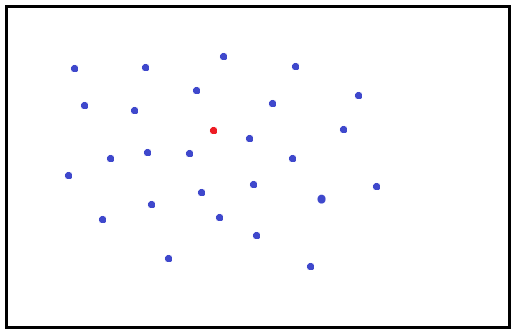
\includegraphics[width=\textwidth]{featurebaggingA.png}
			\caption{The anomaly does not stand out from the data}
			\label{fig:featurebaggingA}
		\end{subfigure}
		\hfill
		\begin{subfigure}[b]{0.49\textwidth}
			\centering
			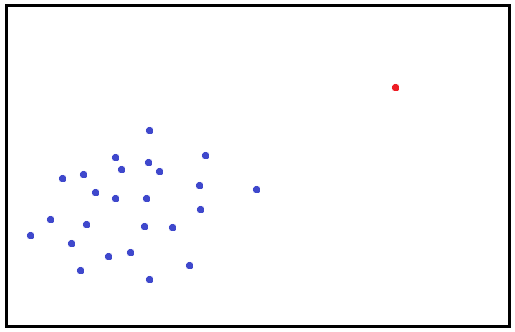
\includegraphics[width=\textwidth]{featurebaggingB.png}
			\caption{The anomaly stands out from the data}
			\label{fig:featurebaggingB}
		\end{subfigure}
		\caption{Two different projections of the data in two dimensions}
		\label{fig:featurebaggingAB}
	\end{figure}
	
	On the other hand if we consider that most dimensions introduce noise into our ensemble, then it is more likely that anomalies will be found through a subset of the dimensions. So this algorithm can be used to be able to detect anomalies by looking at some of the dimensions and not all. In Fig.~\ref{fig:featurebaggingAB} we see exactly this logic, in the first image it seems that we cannot distinguish the anomaly from the rest of the data, but in the second image, we see a projection of the data in two dimensions where the anomaly is isolated.
	
	It is known that the basic algorithms in ensemble techniques must be efficient models but also have a diversity among themselves in order to be able to compose an efficient ensemble model. The ability of the models of course plays an important role, but also the diversity because if the models are different then they will not make the same mistakes and they will be able to capture different pattern in the data. Which means that a mistake made by one model will be covered by the rest. With this method we also manage to give different data sets to the models, therefore each model acquires special characteristics. Thus this algorithm succeeds in differentiating their basic models. The classical bagging algorithm fails to provide an efficient ensemble of basic algorithms based on the local features of the data. This is because such algorithms are not sensitive to sampling methods. However, with feature bagging we succeed in differentiating ourselves from classic bagging in the fact that instead of selecting points, we select features, to which these algorithms are very sensitive, since the selection of features plays an important role in calculating distances.
	
	The procedure for implementing this method is as follows: 
	
	\begin{itemize}
		\item We first take as given a data set $\mathcal{S} = \left\{ X_1, X_2,...X_n \right\}$ where $X_i\in\mathbb{R}^d$, with $d $ be the number of dimensions of $X_i$.
		\item In the first step of the process we select the number of basic algorithms we want to use. Here we have chosen that all the individual algorithms have the same architecture. Let $T$ be their number, for each of them we perform the following steps.
		
		\begin{itemize}
			
			\item We select a random number $N_t$ from a uniform distribution between $\lfloor d \rfloor$ and $(d-1)$. Here $t$ denotes the $t$ algorithm.
			\item Then we randomly select $N_t$ features without repetition and create a set of $\mathcal{F}$ features
			\item We train the anomaly detection algorithm $\text{Alg}_t$ on the data keeping only the $\mathcal{F}$ features.
			\item and we get for each point the anomaly score of the algorithm $t$ $\text{AnomalyScore}_t$
		\end{itemize}
		\item finally for each point we have $ t $ anomaly score (one for each algorithm), \\ $ \text{anomalyscore}_1, \text{anomalyscore}_2, ..., \text{anomalyscore}_t $ \\ and we select the final anomaly score by applying a collection function. That is, \\ $ \text{anomalyscore} = \text{agg} (\text{anomalyscore}_1, \text{anomalyscore}_2, ..., \text {anomalyscore}_t) $.
	\end{itemize}
	
	The choice of collection function also plays an important role in the performance of the algorithm. A well-known one is Breadth-First which selects the item with the highest score of the first algorithm as anomaly, then selects the highest score of the second algorithm as anomaly until it reaches the last algorithm. It then goes to the second largest element of the last algorithm and selects it as an anomaly and does the same until it returns to the first. This process is done until we reach a certain number/percentage of anomalies. This function, although it is very popular, it has the following weakness, it will always find anomalies even if the data set has as few as none, or even if the anomaly scores are very small, until it reaches the required number. Other functions are mean and sum. Here, for our experiments, we have chosen majority voting, which is also used by Random Forests. Finally after selecting a threshold we have the detection of anomalies.
	
	\section{Feature Bagging with Rotation}
	The next method that we implement to increase the performance to detect anomalies for multi variate time series is a generalization of the previous method. The idea has emerged from the well known algorithm called Rotation Forest for the categorization problem {rotation2006Forest} which extends the Random Forest. However, nothing similar has been implemented in the context of detecting abnormalities in multivariate time series (at least in our research).
	
	In order to describe this method we should first make a description of the PCA algorithm. PCA (Principal Component Analysis) is an algorithm known in the literature for dimensionality reduction \cite{han2012mining}. Let $n$ be the dimensions then the algorithm tries to find $k\leq n$ $n\text{-dimensional}$ vectors which are orthogonal to each other and at the same time describe/represent the rest of the data. The data is then projected into the space created by these vectors, thus resulting in a representation of the data in a less dimensional space without losing information. The process is as follows:
	
	\begin{enumerate}
		\item First the data is normalized. Normalizing the data helps prevent very high values from dominating and influencing the result.
		\item For each dimension the average value is calculated.
		\item The correlation matrix (covariance matrix) is then calculated for all dimensions. That is $\text{COV}(X,Y) = \frac{1}{m} \cdot \mathlarger{\sum}\limits_{i=1}^{m}(X-\mu_X)(Y-\ mu_Y) $
		\item Then the eigenvectors and eigenvalues of the previous table are calculated. That is $\text{det}(A-\lambda I) = 0$. These vectors are also called Principal Components while the values represent the "importance".
		\item We put the vectors in descending order according to the eigenvalues. That is, the vector with the largest eigenvalue is entered first, then the one with the next largest eigenvalue etc. The vectors chosen are the $k$ first.
		\item Finally we take the matrix with the eigenvectors and multiply its inverse with the original data matrix to make the conversion, so:
		\[
		\begin{pmatrix}
			\text{new data}
		\end{pmatrix}
		=
		\begin{pmatrix}
			p_1 & ... & p_k
		\end{pmatrix} ^ T
		\begin{pmatrix}
			\text{data}
		\end{pmatrix}		
		\]
	\end{enumerate}
	So we manage to reduce dimensions from $ N $ to $ k $. So if we keep all the eigenvectors and leave no one out it is like turning the axes of the data. This idea enables the model to see the data from another "visual" angle by allowing it to increase its performance. In addition, feature bagging is used to have all the advantages we saw earlier. First we randomly select a subset of all the features then the PCA algorithm is applied to this subset. We get the new data and we train a basic algorithm. This is done for any basic algorithm that the ensemble model is to compose. In the end all results are collected and a collection function is applied. Below we give in detail the procedure followed by the algorithm.
	
	Let $\mathcal{x}$ of size $N$ our data set to make the model training. The $ \mathcal{x}$ have $ n $ dimensions so the data table, say $ A $, is a $ N \ times n $ dimension. Let $ D $ the total of features and $ L $ the multitude of the algorithms to be used. For each basic algorithm we have:
	\begin{itemize}
		\item We select a random number $F_l$ from a uniform distribution between $\lfloor n \rfloor$ and $(n-1)$. Here $l$ denotes the $l$ algorithm.
		\item Then we randomly select without repetition $N_t$ features and create a set of features $F\subseteq D$ and take only these features for our data.
		\item We choose a random number $K$ and divide the set $F$ into $K$ subsets. These subsets may or may not be disjoint. But to increase the diversity between the basic algorithms we choose to be disjoint. Thus the data of each subset consists of $M=n/K$ features.
		\item We choose a percentage of the set $\mathcal{X}$. In the next step we will explain why.
		\item On these subsets we apply PCA and store the coefficients of the principal components, let $a_{l,k}^{1},...a_{l,k}^{M}$, where with $k $ denotes the $k$ subset of $K$. In the previous step we have chosen a percentage of the total. This was done to strengthen the diversity between the coefficients in case the same features are randomly selected between the basic algorithms. So even if the same choices are made by two basic algorithms, the coefficients will be different, and finally we will achieve the diversity we would like.
		\item From the previous step we generate a pivot table for the basic algorithm $l$:
		\[
		R_l = 
		\begin{pmatrix}
			a_{l,1}^{1},...a_{l,1}^{M} & [0] & \cdots & [0] \\
			[0] & a_{l,k}^{1},...a_{l,k}^{M} & \cdots & [0] \\
			\vdots & \vdots & \ddots & \vdots \\
			[0] & [0] & \cdots & a_{l,K}^{1},...a_{l,K}^{M}
		\end{pmatrix}		
		\]
		\item In the previous step we have to pay attention that since the K-subsets have randomly chosen the features $a_i$ are not in order. So in this step we place $a_i$ in the order in which the corresponding features are observed. Let $R^{\text{ordered}}_l$ be a properly ordered matrix.
		\item Finally we get the new data by multiplying $X^l_\text{new} = X_l R^{\text{ordered}}_l$ where $X_l$ is the initial data we would give to the algorithm $l$ before PCA applied. Algorithm $l$ is trained on this data.
		\item As a final step in the process after we have trained $L$ basic algorithms, we apply a collection function. We decided to follow the example of Random Forest and use Majority Voting.
	\end{itemize}
	In this process we will notice that the percentage of the elements we keep to achieve diversity between the basic algorithms and the $ K$ number, are parameters in this ensemble method.
	
	This algorithm as we shall see below seems to give very good results. One disadvantage it has is the many parameters we have to choose. The algorithm, in addition to the parameters of the basic algorithms to be selected, has an additional $ K $ to be selected and the percentage of elements to be selected. In addition, its largest disadvantage is the long training time. Its training time depends on 2 factors. Initially we have the training time of every basic sub-model and then we have the time it takes for the PCA, which is extremely time-consuming. So the time it takes such an ensemble to be trained is quite long.
	
	\section{Stacking Feature Bagging with Rotation Models}
	As we said before, in the technique called Stacking, all models are trained in parallel. Based on the output of the models in the first step, a meta-learner is trained. To implement this technique we use in the first stage, models which built by the Feature Bagging with Rotation method and then we use a Logistic Regressor as a meta-learner. The process is as follows:
	
	\begin{itemize}
		\item First we select a subset of the data on which to train. We divide this subset into two subsets, $A$ and $B$. In $A$ the individual models will be trained while in $B$ the meta-learner will be trained. In this way there is no leak of the information between base models and the meta-learner.
		\item We choose a number $k>1$.
		\item For each base model, $k_n$ models are constructed using the Feature Bagging with Rotation technique as described earlier (where $n$ is the n-th base model).
		\item Each model is trained and produces an anomaly score.
		\item With these individual models we make predictions on data that the models have not been trained on, i.e. on the set $B$. So for each point we get $k_n*n$ features where $k_n$ is the number we chose at the beginning and $n$ is the number of our initial models. Thus a new set is constructed from the data set $B$, let it be $B'$ and for each of its elements we have $b_i = (SA_{k_n,n})_{k_n,n} \in \mathbb{R} ^{k_n \times n}$, where $SA$ denotes the anomaly score given by the $k_n$-th model generated from the n-th base model through the Feature Bagging with Rotation technique.
		\item On set $B'$ we apply supervised learning by training a Logistic Regressor.
	\end{itemize}
	This method combines all of the above and the result is to get a very powerful model as we will see below. The weakness of this technique is that it maintains all the challenges from the above techniques and the training time is much longer.
	
	\section{Architectures, Hyperparameters and Methodology}
	
	Learning for each model is done in each data set individually as well as the prediction. All models are trained in the same data. The final results include the performance aggregated from all data sets. We have also produced results for the basic models so that the comparison can be made between ensemble methods and basic methods. The training is unsupervised (except for techniques that include a logistic regressor that the model is trained with partial surgery) so no model is aware of the information "Anomaly". The "Anomaly" information is used at the end to calculate the performance of each algorithm. The architectural and parameters used in simple models are also applied to models that make up ensemble techniques. Finally, the data does not be pre-processed other than some kind of normalization and the "shuffling" technique does not applied because this would remove the concept of time. In order to compare the algorithms among themselves, the total F1 score and the total AUC (for all data) are calculated for each algorithm while at the same time we provide the confusion table.
	
	Let the data sets (each set is a multivariate time series) can be represented by $(t_0, t_1,....t_n)$ The training set of each data set is from time $t_0$ to time $t_{ 399}$ and the test set is $(t_{400}, t_{401},...t_n)$. In the cases where the Logistic Regressor has been used the training set of the individual models consists of the points $(t_0, t_1,....t_{399})$, the training set with semi-supervised learning of the Logistic Regressor consists of the points $(t_{400}, t_{401},...t_{599})$ and the remaining points are used as tests (The average size of the time series is about ~1100 time points). The basic models we chose are Autoencoder, Convolutional Autoencoder, LSTM, LSTM Autoencoder and LSTM Variational Autoencoder and in Fig.~\ref{fig:plot_model_architecture_model} we can see their architectures.
	
	\begin{figure}[H]
		\begin{subfigure}[b]{0.3\textwidth}
			\centering
			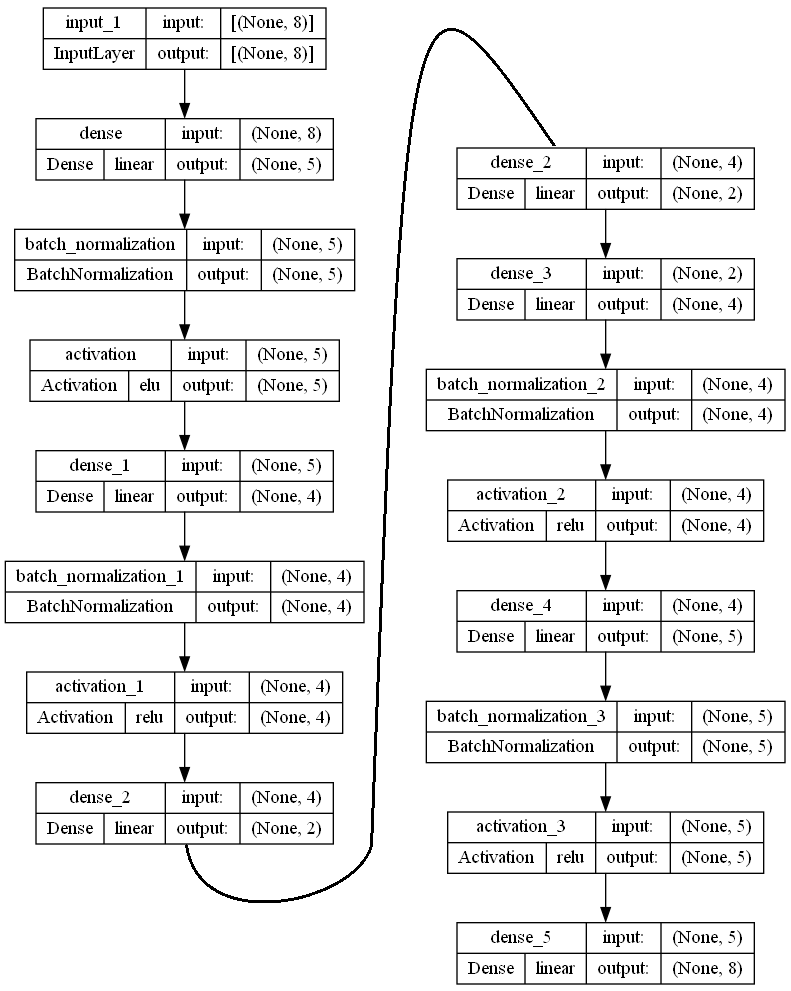
\includegraphics[width=\textwidth]{plot_model_autoencoder_model_c.png}
			\caption{Autoencoder}
			\label{fig:plot_model_autoencoder_model}
		\end{subfigure}
		\hfill
		\begin{subfigure}[b]{0.3\textwidth}
			\centering
			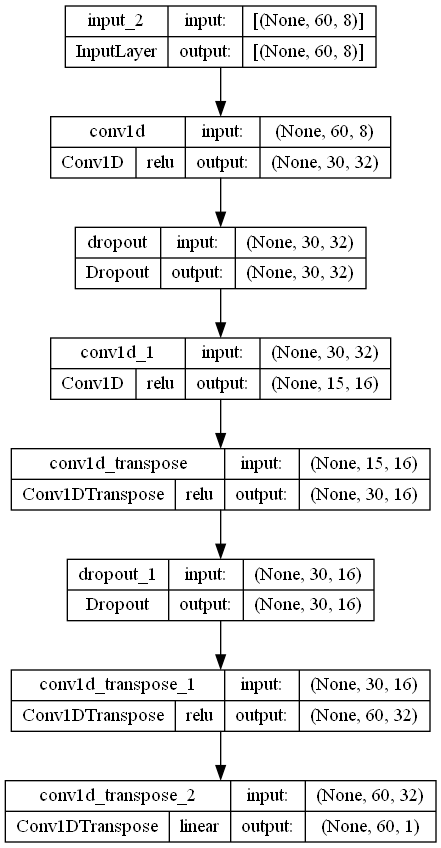
\includegraphics[width=\textwidth]{plot_model_conv_ae_model.png}
			\caption{Convolutional Autoencoder}
			\label{fig:plot_model_conv_ae_model}
		\end{subfigure}
		\hfill
		\begin{subfigure}[b]{0.3\textwidth}
			\centering
			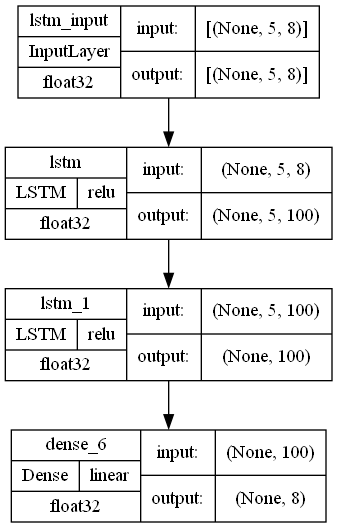
\includegraphics[width=\textwidth]{plot_model_lstm_model.png}
			\caption{LSTM}
			\label{fig:plot_model_lstm_model}
		\end{subfigure}
		\hfill
		\begin{subfigure}[b]{0.3\textwidth}
			\centering
			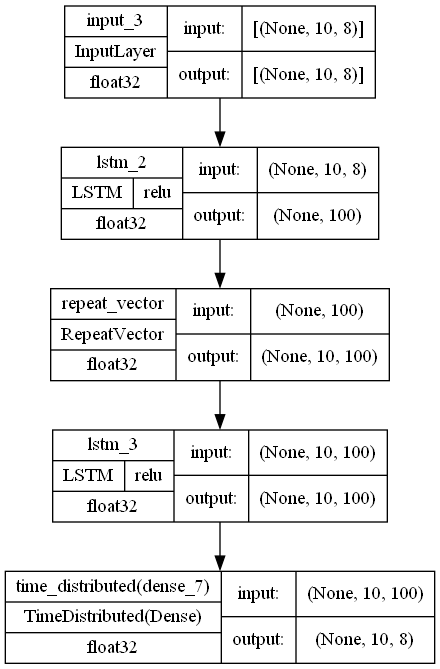
\includegraphics[width=\textwidth]{plot_model_lstm_ae_model.png}
			\caption{LSTM Autoencoder}
			\label{fig:plot_model_lstm_ae_model}
		\end{subfigure}
		\hfill
		\begin{subfigure}[b]{0.5\textwidth}
			\centering
			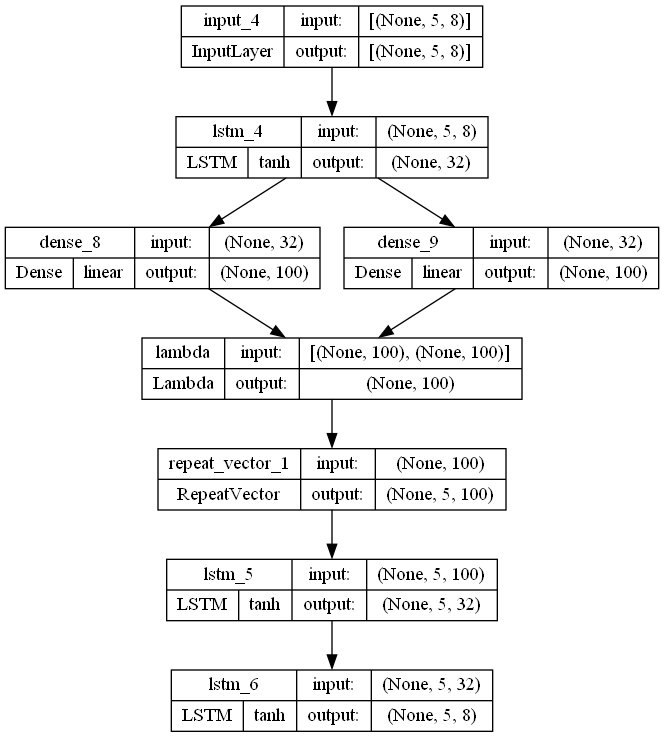
\includegraphics[width=\textwidth]{plot_model_lstm_vae_model.png}'
			\caption{LSTM Variational Autoencoder}
			\label{fig:plot_model_lstm_vae_model}
		\end{subfigure}
		
		\caption{Basic Models Architectures}
		\label{fig:plot_model_architecture_model}
	\end{figure}
	
	The window size we use is 60 time moments for the Convolutional Autoencoder, 5 for the LSTM, 10 for the LSTM Autoencoder, and 5 for the LSTM Variational Autoencoder. For the Feature Bagging technique we used 17 estimators. For the Feature Bagging with Rotation technique, 17 estimators were used, K was set to 2, and the percentage of data used for the PCA algorithm was 75\%. Finally, in the Stacking of Feature Bagging with Rotation with a Logistic Regressor meta-learner, 12 estimators were used for each of the 5 basic algorithms where the parameters for each of them were K=2 and the percentage at 80\%. Let's remember here that the basic techniques and the Majority Voting and Logistic Regression techniques use all the features, while in the rest of the techniques the features that used are based on what we described according to the technique was applied.
	
	\chapter{Results}
	\section{Confusion Matrix}
	The above techniques were applied to 31 datasets simulating different situations. For each of these ensembles the models are trained on a piece of them and then make the predictions on the entire ensembles. In the context of anomaly detection we cannot measure the performance of a model with the classic "Accuracy" metric which is given by $\text{Accuracy} = \frac{\text{TP}+\text{TN}}{\ text{TP}+\text{FP}+\text{TN}+\text{FN}}$ where TP, FP, TN, FN are True Positives, False Positives, True Negatives, False Negatives respectively. So we chose to measure the performance based on F1 score and AUC (the definitions were given in a previous chapter). Next we will give the results from the techniques we mentioned on the data set, but first, we should explain what a Confusion Table is.
	
	\begin{figure}[h]
		\centering
		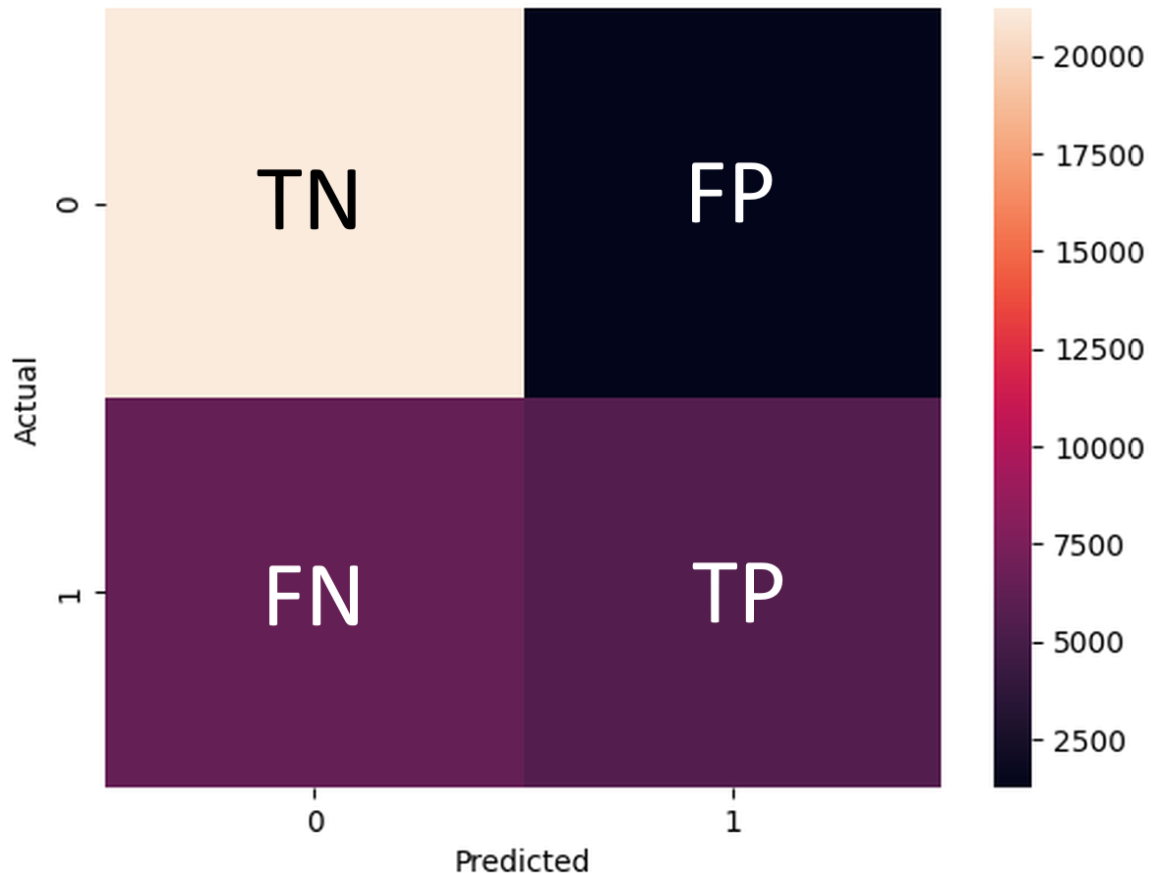
\includegraphics[width=\textwidth/2]{confusionmatrixexplain.png}
		\caption{Confusion Matrix}
		\label{fig:confusionmatrixexplain}
	\end{figure}
	
	A Confusion Table consists of 4 areas True Positives, True Negatives, False Positives and False Negatives. On the left side of the table we can choose between the real data (top line the real normal points while in the bottom line we have the real Abnormal data). On the lower side of the table we can choose between the predictions (in the left column we have the predictions of the normal points while on the right the predictions of the abnormal points). In Fig.~\ref{fig:confusionmatrixexplain} we see a confusion matrix where instead of numbers we have noted in each area what it shows. We note here that the ideal model would have in the regions of FP and FN the number zero.
	
	\begin{figure}[H]
		\centering
		\begin{subfigure}[b]{0.35\textwidth}
			\centering
			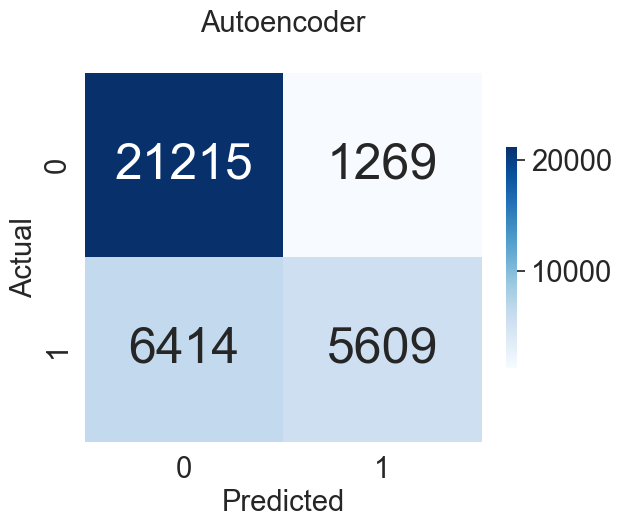
\includegraphics[width=\textwidth]{anomaly_by_autoencoder.png}
			
			\label{fig:anomaly_by_autoencoder}
		\end{subfigure}
		\hfil
		\begin{subfigure}[b]{0.35\textwidth}
			\centering
			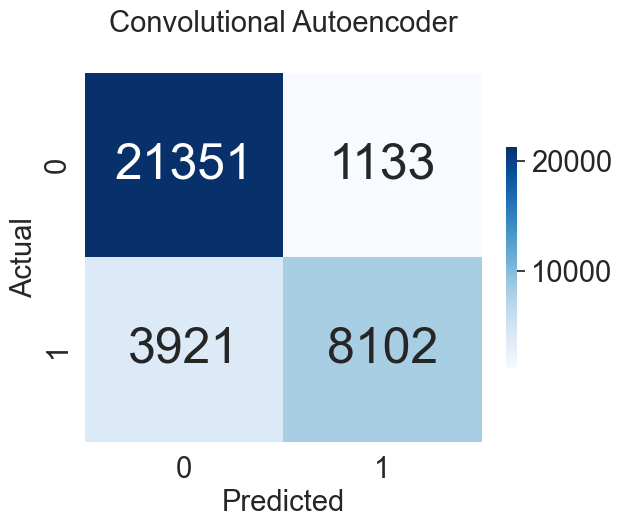
\includegraphics[width=\textwidth]{anomaly_by_conv_ae.png}
			
			\label{fig:anomaly_by_conv_ae}
		\end{subfigure}
		\bigskip
		\begin{subfigure}[b]{0.35\textwidth}
			\centering
			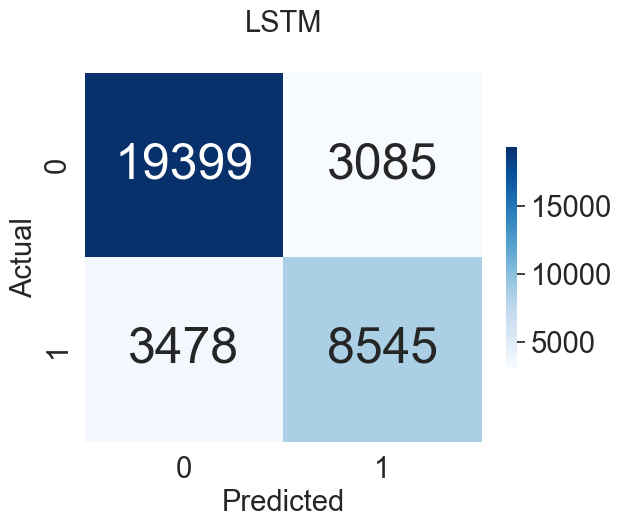
\includegraphics[width=\textwidth]{anomaly_by_lstm.png}
			
			\label{fig:anomaly_by_lstm}
		\end{subfigure}
		\hfil
		\begin{subfigure}[b]{0.35\textwidth}
			\centering
			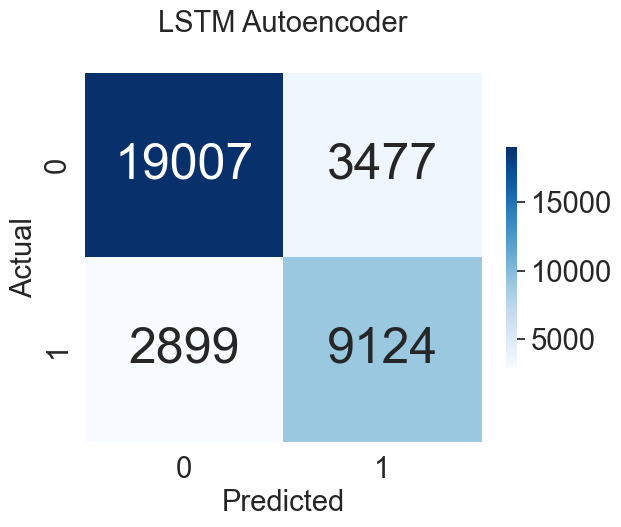
\includegraphics[width=\textwidth]{anomaly_by_lstm_ae.png}
			
			\label{fig:anomaly_by_lstm_ae}
		\end{subfigure}
		\medskip
		\begin{subfigure}[b]{0.35\textwidth}
			\centering
			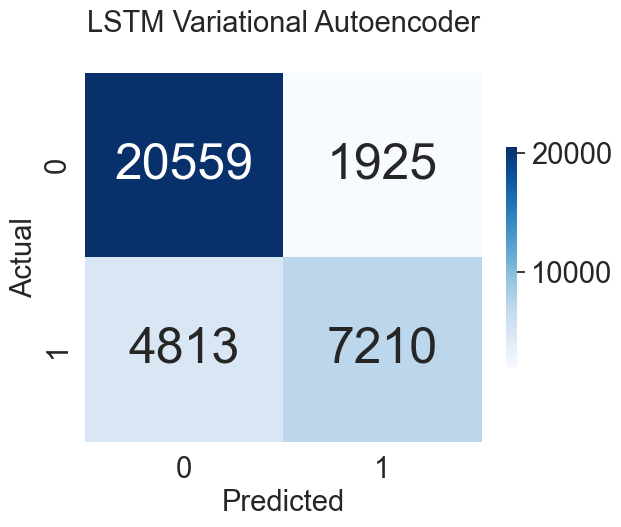
\includegraphics[width=\textwidth]{anomaly_by_lstm_vae.png}
			
			\label{fig:anomaly_by_lstm_vae}
		\end{subfigure}
		\caption{Basic Models}
		\label{fig:basicmodelsconfusion}
	\end{figure}
	
	Along with the techniques, we also trained the basic models so that we have a measure of comparison afterwards. In Fig.~\ref{fig:basicmodelsconfusion} we see the results that the basic models had. We observe that the models achieve good performance especially the convolutional autoencoder and the LSTM autoencoder.
	
	\begin{figure}[H]
		\centering
		\begin{subfigure}[b]{0.35\textwidth}
			\centering
			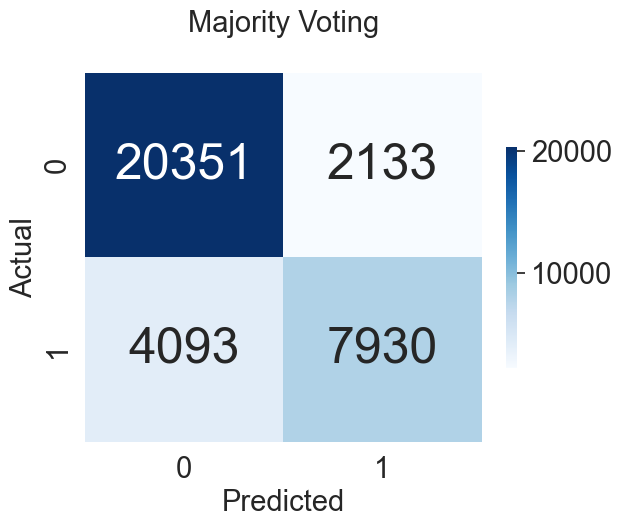
\includegraphics[width=\textwidth]{anomaly_by_voting.png}
			
			\label{fig:anomaly_by_voting}
		\end{subfigure}
		\hfil
		\begin{subfigure}[b]{0.35\textwidth}
			\centering
			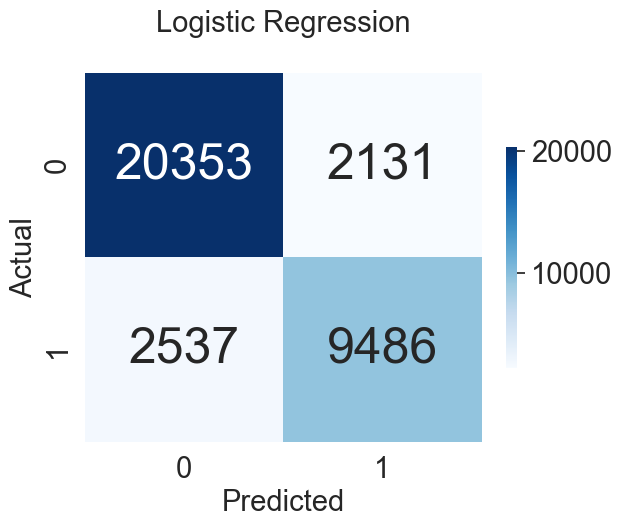
\includegraphics[width=\textwidth]{anomaly_by_logistic_regression.png}
			
			\label{fig:anomaly_by_logistic_regression}
		\end{subfigure}
		\caption{Majority Voting - Logistic Regression}
		\label{fig:majoritylogistic}
	\end{figure}
	
	
	\begin{figure}[H]
		\centering
		\begin{subfigure}[b]{0.35\textwidth}
			\centering
			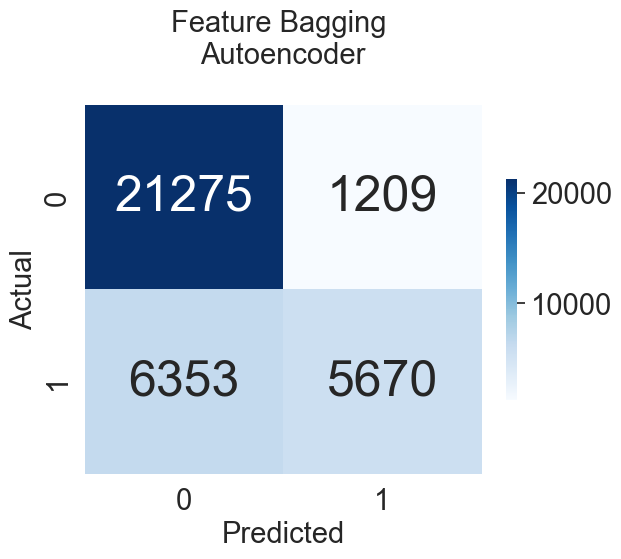
\includegraphics[width=\textwidth]{anomaly_by_ensemble_ensemble_autoencoder.png}
			
			\label{fig:anomaly_by_ensemble_ensemble_autoencoder}
		\end{subfigure}
		\hfil
		\begin{subfigure}[b]{0.35\textwidth}
			\centering
			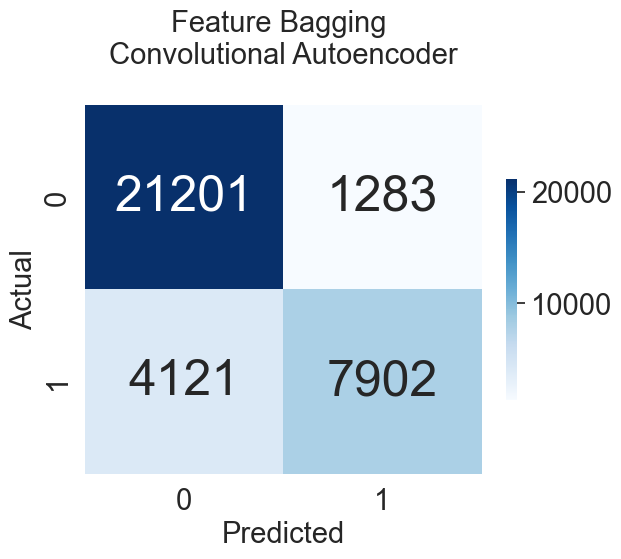
\includegraphics[width=\textwidth]{anomaly_by_ensemble_ensemble_conv_ae.png}
			
			\label{fig:anomaly_by_ensemble_ensemble_conv_ae}
		\end{subfigure}
		\medskip
		\begin{subfigure}[b]{0.35\textwidth}
			\centering
			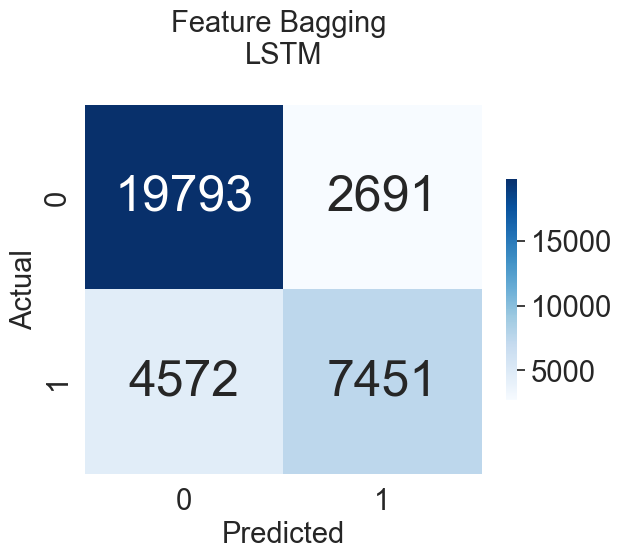
\includegraphics[width=\textwidth]{anomaly_by_ensemble_ensemble_lstm.png}
			
			\label{fig:anomaly_by_ensemble_ensemble_lstm}
		\end{subfigure}
		\hfil
		\begin{subfigure}[b]{0.35\textwidth}
			\centering
			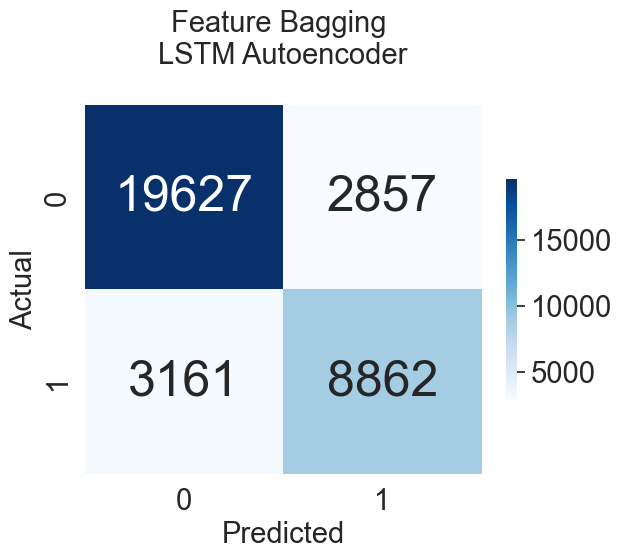
\includegraphics[width=\textwidth]{anomaly_by_ensemble_ensemble_lstm_ae.png}
			
			\label{fig:anomaly_by_ensemble_ensemble_lstm_ae}
		\end{subfigure}
		\medskip
		\begin{subfigure}[b]{0.35\textwidth}
			\centering
			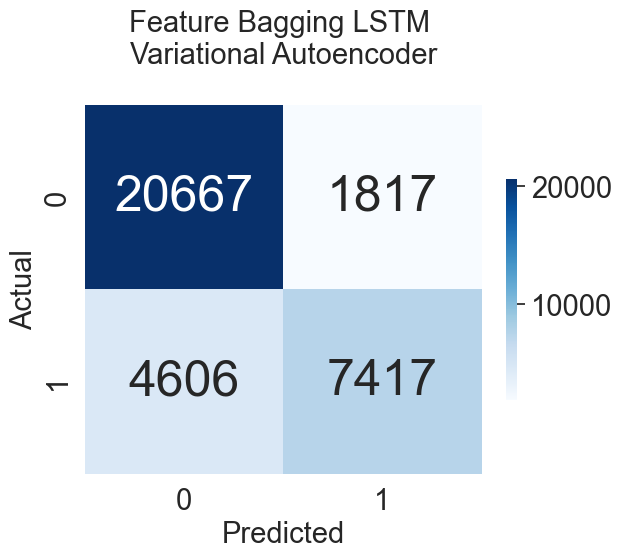
\includegraphics[width=\textwidth]{anomaly_by_ensemble_ensemble_lstm_vae.png}
			
			\label{fig:anomaly_by_ensemble_ensemble_lstm_vae}
		\end{subfigure}
		\caption{Feature Bagging}
		\label{fig:featurebaggingmodelsconfusion}
	\end{figure}
	
	Then we give the results for the techniques we mentioned earlier. We start with Majority Voting and the technique where we apply semi-supervised learning with logistic regression fig.~\ref{fig:majoritylogistic}. We notice that both algorithms are very close to the points that are not abnormalities but differ in abnormal points. As we can see, Logistic Regression achieves better results there.
	
	Then we present the results of the Feature Bagging technique Fig.~\ref{fig:featurebaggingmodelsconfusion}. We observe that there is a variety of results here depending on the basic algorithm used. In the next section we will see a comparison between each basic algorithm and the technique of feature baging that corresponds to it.
	
	\begin{figure}[H]
		\centering
		\begin{subfigure}[b]{0.35\textwidth}
			\centering
			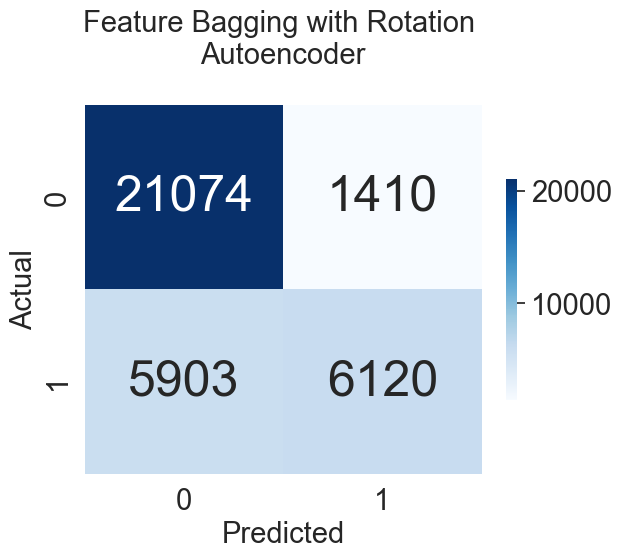
\includegraphics[width=\textwidth]{anomaly_by_ensemble_ensemble_rotation_autoencoder.png}
			
			\label{fig:anomaly_by_ensemble_ensemble_rotation_autoencoder}
		\end{subfigure}
		\hfil
		\begin{subfigure}[b]{0.35\textwidth}
			\centering
			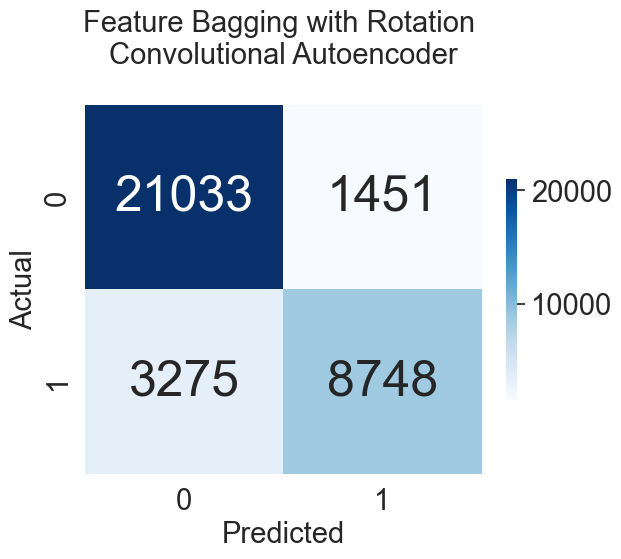
\includegraphics[width=\textwidth]{anomaly_by_ensemble_ensemble_rotation_conv_ae.png}
			
			\label{fig:anomaly_by_ensemble_ensemble_rotation_conv_ae}
		\end{subfigure}
		\medskip
		\begin{subfigure}[b]{0.35\textwidth}
			\centering
			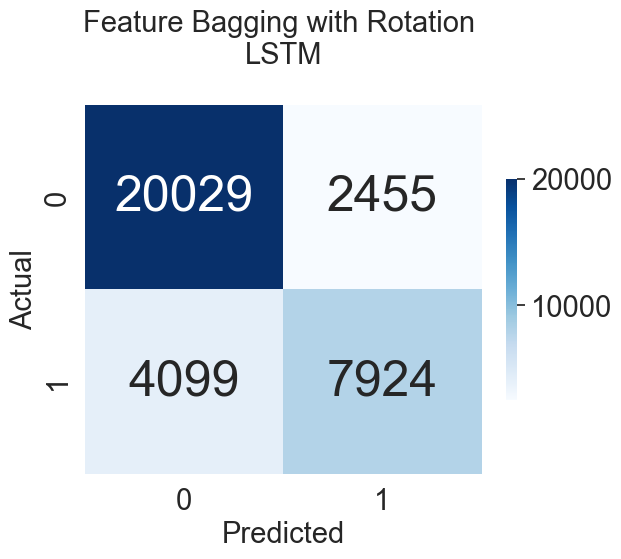
\includegraphics[width=\textwidth]{anomaly_by_ensemble_ensemble_rotation_lstm.png}
			
			\label{fig:anomaly_by_ensemble_ensemble_rotation_lstm}
		\end{subfigure}
		\hfil
		\begin{subfigure}[b]{0.35\textwidth}
			\centering
			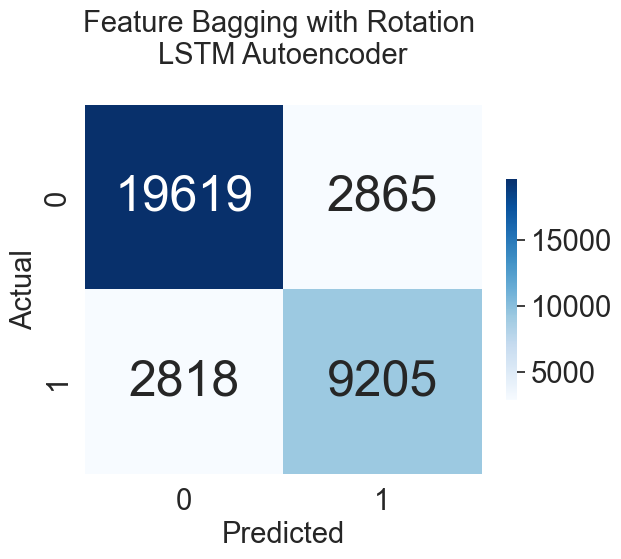
\includegraphics[width=\textwidth]{anomaly_by_ensemble_ensemble_rotation_lstm_ae.png}
			
			\label{fig:anomaly_by_ensemble_ensemble_rotation_lstm_ae}
		\end{subfigure}
		\medskip
		\begin{subfigure}[b]{0.35\textwidth}
			\centering
			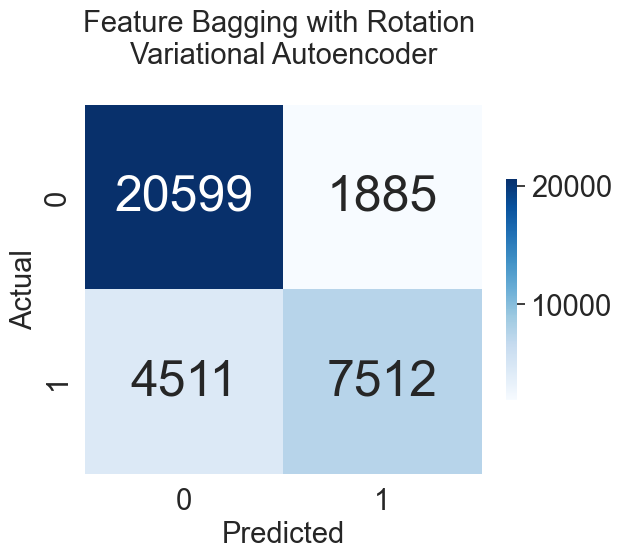
\includegraphics[width=\textwidth]{anomaly_by_ensemble_ensemble_rotation_lstm_vae.png}
			
			\label{fig:anomaly_by_ensemble_ensemble_rotation_lstm_vae}
		\end{subfigure}
		\caption{Feature Bagging with Rotation}
		\label{fig:featurebaggingwithrotationmodelsconfusion}
	\end{figure}
	
	In Fig.~\ref{fig:featurebaggingwithrotationmodelsconfusion} we present the results of the Feature Bagging with Rotation technique where with the help of the PCA algorithm we turn the axes. We notice here, that depending on the basic algorithm that has been used there is a variety in the results, but generally this techniques performs well.
	
	\begin{figure}[H]
		\centering
		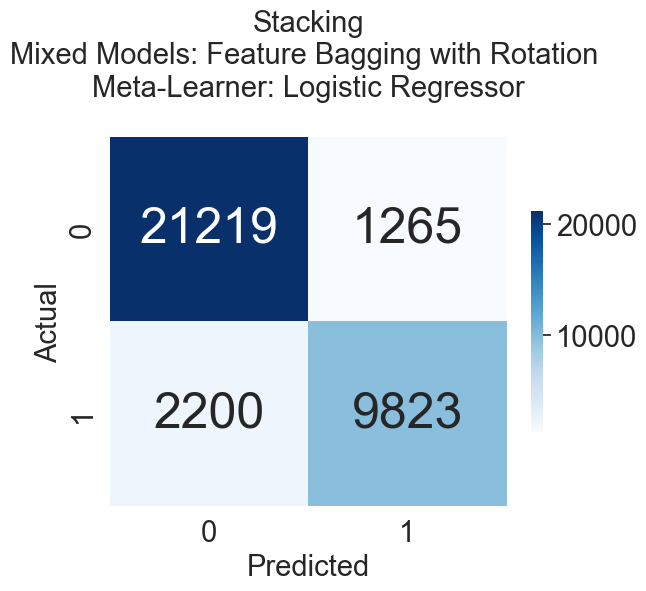
\includegraphics[width=\textwidth/2]{anomaly_by_logistic_regression_mixed_models.png}
		\caption{Stacking, Mixed Models: Feature Bagging with Rotation, Meta-Learner: Logistic Regressor}
		\label{fig:anomaly_by_logistic_regression_mixed_models}
	\end{figure}
	
	Finally we list the results from the Stacking we used on models made by the Feature Bagging with Rotation technique with a Logistic Regressor meta-model Fig.~\ref{fig:anomaly_by_logistic_regression_mixed_models}.
	
	\section{Comparisons based on F1 and AUC Score}
	
	The tables below show a comparison between basic models and ensemble techniques. As we said before, we use the F1 Score and AUC metrics to evaluate the models. Based on these metrics we notice that the Feature Bagging technique gives quite good results in some cases while the technique of Feature Bagging with Rotation earns in all comparisons except if the basic model is LSTM. In addition, Majority Voting is about in the middle (which we expected because it relies on the majority) while the algorithm with the logistic regression wins the basic algorithms as it relies on learning to make the best choice based on prediction that the basic methods feed to it. In addition, it is the only algorithm that knows at least a few labels from the data. Finally, it is worth noting that we cannot make comparisons between feature bagging techniques because they do not rely on the same basic algorithms. The same is true with the technique of feature baging with rotation. Finally we observe that the advantages of Logistic Regression applies to the last algorithm which take advantage of Feature Bagging with Rotation models through stacking them. The Logistic Regressor we used as a meta-learner gives us the best performance which it was expected because the simpler method of the above Logistic Regression above performed very well on the basic models.
	
	\begin{table}[H]
		\centering
		\resizebox{\textwidth/3*2}{!}{
			\begin{tabular}{|c|c|c|}
				\hline
				Model Title & F1 Score & AUC \\
				\hline
				Feature Bagging with Rotation Autoencoder & 62.59 \% & 72.31 \% \\
				%& 0.6259908965376157 & 0.7231565543080914 \\
				\hline
				Feature Bagging Autoencoder & 59.99 \% & 70.89 \% \\
				% & 0.5999365146545339 & 0.7089122682829209 \\
				\hline
				Autoencoder & 59.35 \% & 70.50 \% \\ 
				% & 0.5935135707105444 & 0.705041181668599 \\
				\hline
			\end{tabular}
		}
		\caption{Autoencoder}
		\label{tab:comptabautoencoder}
	\end{table}
	
	We observe that Autoencoder, LSTM Autoencoder and LSTM Variational Autoencoder Feature Bagging have better performance than the corresponding basic model and Feature Bagging with Rotation better performance than Feature Bagging. The FBR algorithm achieves an improvement of 2 \% compared to the basic models Table~\ref{tab:comptabautoencoder}, Table~\ref{tab:comptablstmautoencoder},  Table~\ref{tab:comptablstmvariationlautoencoder}. In the case of Convolutional Autoencoder, the feature baging with rotation continues to perform better but unlike the previous ones the algorithm Feature Bagging does not, Table~\ref{tab:comptabconvolutionalautoencoder}. The only basic algorithm that has better performance than the corresponding versions of Feature Bagging and Feature Bagging With Rotation is the LSTM Table~\ref{tab:comptablstm}. The comparison between these two techniques shows us that FBR method performs better than Feature Bagging in all cases.

	It is worth to remind here that every Feature Bagging technique consist of models with the corresponding architecture. The same applies to Feature Bagging with Rotation algorithm. So for example in the case of LSTM Autoencoder, only LSTM Autoencoders created to compose an LSTM Autoencoder ensemble Feature Bagging. Furthermore the training was done with 17 estimators for each case in the Feature Bagging and the FBR techniques. Additionally in FBR technique we used K=2 and a percentage of data at 75 \%. 
	
	\begin{table}[H]
		\centering
		\resizebox{\textwidth}{!}{
			\begin{tabular}{|c|c|c|}
				\hline
				Model Title & F1 Score & AUC \\
				\hline
				Feature Bagging with Rotation Convolutional Autoencoder & 78.73 \%  & 83.15 \% \\
				% & 0.7873278732787328 & 0.8315353213255807 \\
				\hline
				Convolutional Autoencoder & 76.22 \% & 81.17 \% \\
				% & 0.7622542101796971 & 0.8117418416723458 \\
				\hline
				Feature Bagging Convolutional Autoencoder & 74.51 \% & 80.00 \% \\
				% & 0.7451904941531498 & 0.8000887446158723 \\
				\hline
			\end{tabular}
		}
		\caption{Convolutional Autoencoder}
		\label{tab:comptabconvolutionalautoencoder}
	\end{table}
	
	\begin{table}[H]
		\centering
		\resizebox{\textwidth/3*2}{!}{
			\begin{tabular}{|c|c|c|}
				\hline
				Model Title & F1 Score & AUC \\
				\hline
				LSTM & 72.25 \% & 78.67 \% \\
				% & 0.7225299116391154 & 0.786756218064105 \\
				\hline
				Feature Bagging with Rotation LSTM & 70.74 \% & 77.49 \% \\
				% & 0.707436835996786 & 0.7749406795813568 \\
				\hline
				Feature Bagging LSTM & 67.23 \% & 75.00 \% \\
				% & 0.6723212271599368 & 0.7500218718102761 \\
				\hline
			\end{tabular}
		}
		\caption{LSTM}
		\label{tab:comptablstm}
	\end{table}
	
	\begin{table}[H]
		\centering
		\resizebox{\textwidth/3*2}{!}{
			\begin{tabular}{|c|c|c|}
				\hline
				Model Title & F1 Score & AUC \\
				\hline
				Feature Bagging with Rotation LSTM Autoencoder & 76.41 \% & 81.90 \% \\ 
				% & 0.7641223591914665 & 0.8190959784678844 \\
				\hline
				Feature Bagging LSTM Autoencoder & 74.65 \% & 80.50 \% \\
				% & 0.7465251453121052 & 0.805009556048233 \\
				\hline
				LSTM Autoencoder & 74.10 \% & 80.21 \% \\
				% & 0.7410656270305394 & 0.8021177568499255 \\
				\hline
			\end{tabular}
		}
		\caption{LSTM Autoencoder}
		\label{tab:comptablstmautoencoder}
	\end{table}
	
	\begin{table}[H]
		\centering
		\resizebox{\textwidth/4*3}{!}{
			\begin{tabular}{|c|c|c|}
				\hline
				Model Title & F1 Score & AUC \\
				\hline
				Feature Bagging with Rotation LSTM Variational Autoencoder & 70.14 \% & 77.04 \% \\
				% & 0.7014005602240897 & 0.770482533233351 \\
				\hline
				Feature Bagging LSTM Variational Autoencoder & 69.78 \% & 76.80 \% \\
				% & 0.6978407112951028 & 0.768043958635707 \\
				\hline
				LSTM Variational Autoencoder & 68.15 \% & 75.70 \% \\
				% & 0.6815388978164287 & 0.7570337503802643 \\
				\hline
			\end{tabular}
		}
		\caption{LSTM Variational Autoencoder}
		\label{tab:comptablstmvariationalautoencoder}
	\end{table}
	
	Majority Voting is placed in the middle of the table with a slight difference from LSTM while at the same time it has achieved a better performance than Autoencoder by more than 8\% Table~\ref{tab:comptablstm}. In Majority Voting five models are used (the five models we described earlier). Every model's prediction weighted equal to the others and the prediction is made according the majority.
	
	\begin{table}[H]
		\centering
		\resizebox{\textwidth/2}{!}{
			\begin{tabular}{|c|c|c|}
				\hline
				Model Title & F1 Score & AUC \\
				\hline
				Convolutional Autoencoder & 76.22 \% & 81.17 \% \\
				% & 0.7622542101796971 & 0.8117418416723458 \\
				\hline
				LSTM Autoencoder & 74.10 \% & 80.21 \% \\
				% & 0.7410656270305394 & 0.8021177568499255 \\
				\hline
				LSTM & 72.25 \% & 78.67 \% \\
				% & 0.7225299116391154 & 0.786756218064105 \\
				\hline
				Majority Voting & 71.81 \% & 78.23 \% \\
				% & 0.7181019650457303 & 0.7823508489029425 \\
				\hline
				LSTM Variational Autoencoder & 68.15 \% & 75.70 \% \\
				% & 0.6815388978164287 & 0.7570337503802643 \\
				\hline
				Autoencoder & 59.35 \% & 70.50 \% \\
				% & 0.5935135707105444 & 0.705041181668599 \\
				\hline
			\end{tabular}
		}
		\caption{Majority Voting}
		\label{tab:comptabmajorityvoting}
	\end{table}
	
	
	In Table~\ref{tab:comptablogreg} we notice that Logistic Regressor achieves better results than all basic algorithms. This indicates that Logistic Regressor can combine efficiently the different algorithms. We remind that all five models were used in this technique. The five models were trained on a set A and the Logistic Regressor on a set B (Logistic Regression was trained on the predictions of the five models of the set B) where A and B do not share any information (they are disjoint). This decision taken in order to prevent information leakage.  
	
	\begin{table}[H]
		\centering
		\resizebox{\textwidth/2}{!}{
			\begin{tabular}{|c|c|c|}
				\hline
				Model Title & F1 Score & AUC \\
				\hline
				Logistic Regression & 80.25 \% & 84.71 \% \\
				% & 0.8025380710659897 & 0.8471046321360901 \\
				\hline
				Convolutional Autoencoder & 76.22 \% & 81.17 \% \\
				% & 0.7622542101796971 & 0.8117418416723458 \\
				\hline
				LSTM Autoencoder & 74.10 \% & 80.21 \% \\
				% & 0.7410656270305394 & 0.8021177568499255 \\
				\hline
				LSTM & 72.25 \% & 78.67 \% \\
				% & 0.7225299116391154 & 0.786756218064105 \\
				\hline
				LSTM Variational Autoencoder & 68.15 \% & 75.70 \% \\
				% & 0.6815388978164287 & 0.7570337503802643 \\
				\hline
				Autoencoder & 59.35 \% & 70.50 \% \\
				% & 0.5935135707105444 & 0.705041181668599 \\
				\hline
			\end{tabular}
		}
		\caption{Logistic Regression}
		\label{tab:comptablogreg}
	\end{table}
	
	Finally the best performance is achieved from when we use the Stacking method on Feature Bagging with Rotation models with meta-learner a Logistic Regressor Table~\ref{tab:comptablogregmixedmodels}. Because on the above results we saw that Feature Bagging with Rotation perform well compared to the Feature Bagging and the basic models and because of the Logistic Regressor which can combine pretty well the basic models we decided to compose an ensemble from these two components. So we created 12 models from each of the basic models with the FBR technique (meaning 12 models from LSTM with FBR technique, 12 models from Autoencoder with FBR technique etc) and we fed a Logistic Regressor. Again the training of individual models was done on a set A and the training of the Logistic Regressor on a set B, where A and B are disjoint, in order to avoid information leakage. The other parameters of the FBR methods, $K$ and the percentage of data, were set to 2 and 80 \% respectively. 
	
	\begin{table}[H]
		\centering
		\resizebox{\textwidth/2}{!}{
			\begin{tabular}{|c|c|c|}
				\hline
				Model Title & F1 Score & AUC \\
				\hline
				Stacking with Logistic Regression & 85.00 \% & 88.03 \% \\
				% & 0.8025380710659897 & 0.8471046321360901 \\
				\hline
				Convolutional Autoencoder & 76.22 \% & 81.17 \% \\
				% & 0.7622542101796971 & 0.8117418416723458 \\
				\hline
				LSTM Autoencoder & 74.10 \% & 80.21 \% \\
				% & 0.7410656270305394 & 0.8021177568499255 \\
				\hline
				LSTM & 72.25 \% & 78.67 \% \\
				% & 0.7225299116391154 & 0.786756218064105 \\
				\hline
				LSTM Variational Autoencoder & 68.15 \% & 75.70 \% \\
				% & 0.6815388978164287 & 0.7570337503802643 \\
				\hline
				Autoencoder & 59.35 \% & 70.50 \% \\
				% & 0.5935135707105444 & 0.705041181668599 \\
				\hline
			\end{tabular}
		}
		\caption{Stacking with Logistic Regression}
		\label{tab:comptablogregmixedmodels}
	\end{table}
	
	
	
	\chapter{Conclusions}
	\section{Conclusions and extension of the work}
	In this work we implemented several ensemble techniques for anomaly detection in multivariate time series. This problem has been approached by various algorithms both from statistical techniques and from Machine learning and deep machine learning models. We took some basic deep machine learning models and built on them to implement ensemble techniques to achieve even better results. The ensemble models built initially were a Majority Voting which had a moderate performance and a semi-supervised training algorithm where a Logistic Regressor was used as the final model. An algorithm called Feature Bagging was then implemented which is very similar to the technique used in Random Forests. Feature Bagging gave some good results in some cases against the base models. Then, from an idea derived from Rotation Forest, PCA was used on Feature Bagging, resulting in an algorithm that in most cases performed better than all of the above and the basic algorithms. Finally, a stacking technique was used with individual models made by the Feature Bagging with Rotation technique and a Logistic Regressor as a meta-learner where we got the best performance from all the previous techniques. Ensemble techniques are known to greatly improve performance and solve many problems. The above results show us that they can also help a lot in detecting anomalies. With the ensemble methods we can go far beyond the simple models and produce a hyper-model which will detect the anomalies quite reliably. In particular, the Feature Bagging with Rotation algorithm was able to perform 2\% better than the base models in some cases, while Feature Bagging when better than a simple model had a better performance of about 1\% in one case, while in the other two it had less than 1\% Finally when we applied Stacking we achieved about 10 \% better performance than the base models. Furthermore Stacking FBR models outperforms any other technique we used.
	
	From the above we can say that it is worth further expanding the work and trying to detect anomalies with ensemble techniques as it seems that ensemble models can provide solutions. Most of the techniques need some function to aggregate the results so this could be the subject of research so that with the appropriate function the results of the basic models can be combined more efficiently. Shahzad and Lavesson have done a research \cite{shahzad2013comparative} in which they investigate variants of Majority Voting and it seems that Majority Voting achieves better results as an algorithm but it would be interesting to investigate whether the variants can be used as selection functions of the techniques we described and whether they can give better results.
	
	In addition, the datasets consist of few features, i.e. the time series of many variables consist of few variables (8 in total), this means that these algorithms could be investigated in higher dimensions. As the dimensions increase, the meaning of the anomaly is lost, which makes it difficult to detect, but we believe that these algorithms could cope very well, especially the Feature Bagging and Feature Bagging with Rotation algorithms, which can take advantage of the many dimensions.
	
	Another important part of these algorithms is the speed part. We noticed that as the complexity increases, so does the time it takes the models to train. This means that it is impossible to go to a very large number of base models. The large number of base models would have allowed us to have better performance but this was impossible given the time it took for example Feature Bagging with Rotation to train. So it is worth investigating further how this could be done in much less time so that such an algorithm could consist of many small basic models.
	
	
	
	\bibliographystyle{ieeetr}
	\bibliography{mybib}
	%\bibliographystyle{abbrv}
	%\bibliographystyle{acm}
	%\bibliographystyle{alpha}
	%\bibliographystyle{apalike}
	%\bibliographystyle{ieeetr}
	%\bibliographystyle{plain}
	%\bibliographystyle{unsrt}
	
\end{document}

